%% Template article for cas-sc documentclass for 
%% single column output.

%\documentclass[a4paper,fleqn,longmktitle]{cas-sc}
% \documentclass[a4paper,fleqn]{cas-sc}
\documentclass[a4paper,fleqn]{cas-sc}

\usepackage[numbers]{natbib}
%\usepackage[authoryear]{natbib}
% \usepackage[authoryear,longnamesfirst]{natbib}
\usepackage{makecell}
\usepackage{tabularx}
\usepackage{multirow}
\usepackage{array}
\usepackage{algorithm}   % 提供 algorithm 浮动体（可选但推荐）
\usepackage{algpseudocode} % 提供 algorithmic 环境

%%%Author macros
\def\tsc#1{\csdef{#1}{\textsc{\lowercase{#1}}\xspace}}
\tsc{WGM}
\tsc{QE}
\tsc{EP}
\tsc{PMS}
\tsc{BEC}
\tsc{DE}
%%%

\begin{document}
\let\WriteBookmarks\relax
\def\floatpagepagefraction{1}
\def\textpagefraction{.001}
\shorttitle{Chain-Structured BNN NAS}
\shortauthors{W.R. et~al.}
%\begin{frontmatter}

\title [mode = title]{Chain-Structured Binary Neural Architecture Search for Efficient Visual Recognition across Platforms}                      


\author[1,2]{Rui Wan}[style=chinese,
    orcid=0009-0007-2606-0334]
\ead{22110093@bjtu.edu.cn}
\credit{Writing–review \& editing, Writing–original draft, Validation, Supervision, Software, Methodology, Investigation, Conceptualization}

\author[1,2]{Dong Wang}[style=chinese]
\cormark[1]
\ead{wangdong@bjtu.edu.cn}
\credit{Writing–review \& editing, Writing–original draft, Visualization, Validation, Methodology, Conceptualization.}

\author[1,2]{Yiwen Liang}[style=chinese]
\credit{Writing–review \& editing, Investigation}

\author[1,2]{Mingrun Wei}[style=chinese]
\credit{Writing–review \& editing, Investigation}

\affiliation[1]{organization={Institute of Information Science},
            addressline={Beijing Jiaotong University}, 
            city={Beijing},
            postcode={100044}, 
            country={China}}

\affiliation[2]{organization={Beijing Key Laboratory of Advanced Information Science and Network Technology},
            city={Beijing},
            postcode={100044}, 
            country={China}}
\cortext[cor1]{Corresponding author}

\begin{abstract}
Neural architecture search (NAS) has been widely used to design accurate binary neural networks (BNNs), spanning both cell-based designs and chain-structured architectures. Despite strong accuracy on large-scale benchmarks, enabling efficient visual recognition with chain-structured BNNs across heterogeneous platforms remains challenging because (1) cross-platform adaptation typically requires expensive per-device searches and (2) BNN latency optimization is often guided by proxy costs (e.g., FLOPs) rather than measured real-device latency. 
To address these issues, we present FlashNAS-BNN, \textcolor{red}{a chain-structured binary NAS framework for efficient search and deployment.} For search efficiency, we combine a chain information-flow accuracy predictor (CIF-Net) with a two-stage search strategy that reuses accuracy-screened candidates and avoids evaluating clearly suboptimal designs on each device. For deployment efficiency, we introduce cross-platform latency estimation (CLE), which improves latency prediction across diverse hardware platforms and robustly identifies latency-optimized architectures.
\textcolor{red}{Experimental results show that FlashNAS-BNN incurs a lower cumulative cost, including offline preparation, than independent NAS-BNN searches for three or more target platforms.} FlashNAS-BNN also achieves consistent latency optimization across CPU, GPU, and FPGA. \textcolor{red}{It reduces latency by 47.1\%, 16.0\%, and 6.8\% over ReActNet-A, and by 39.6\%, 10.6\%, and 8.6\% over corresponding platform-optimized NAS-BNN architectures, on CPU, GPU, and FPGA, respectively, at comparable accuracy.} Code is available at \url{https://github.com/WanRui37/FlashNAS-BNN}.
\end{abstract}

\begin{graphicalabstract}
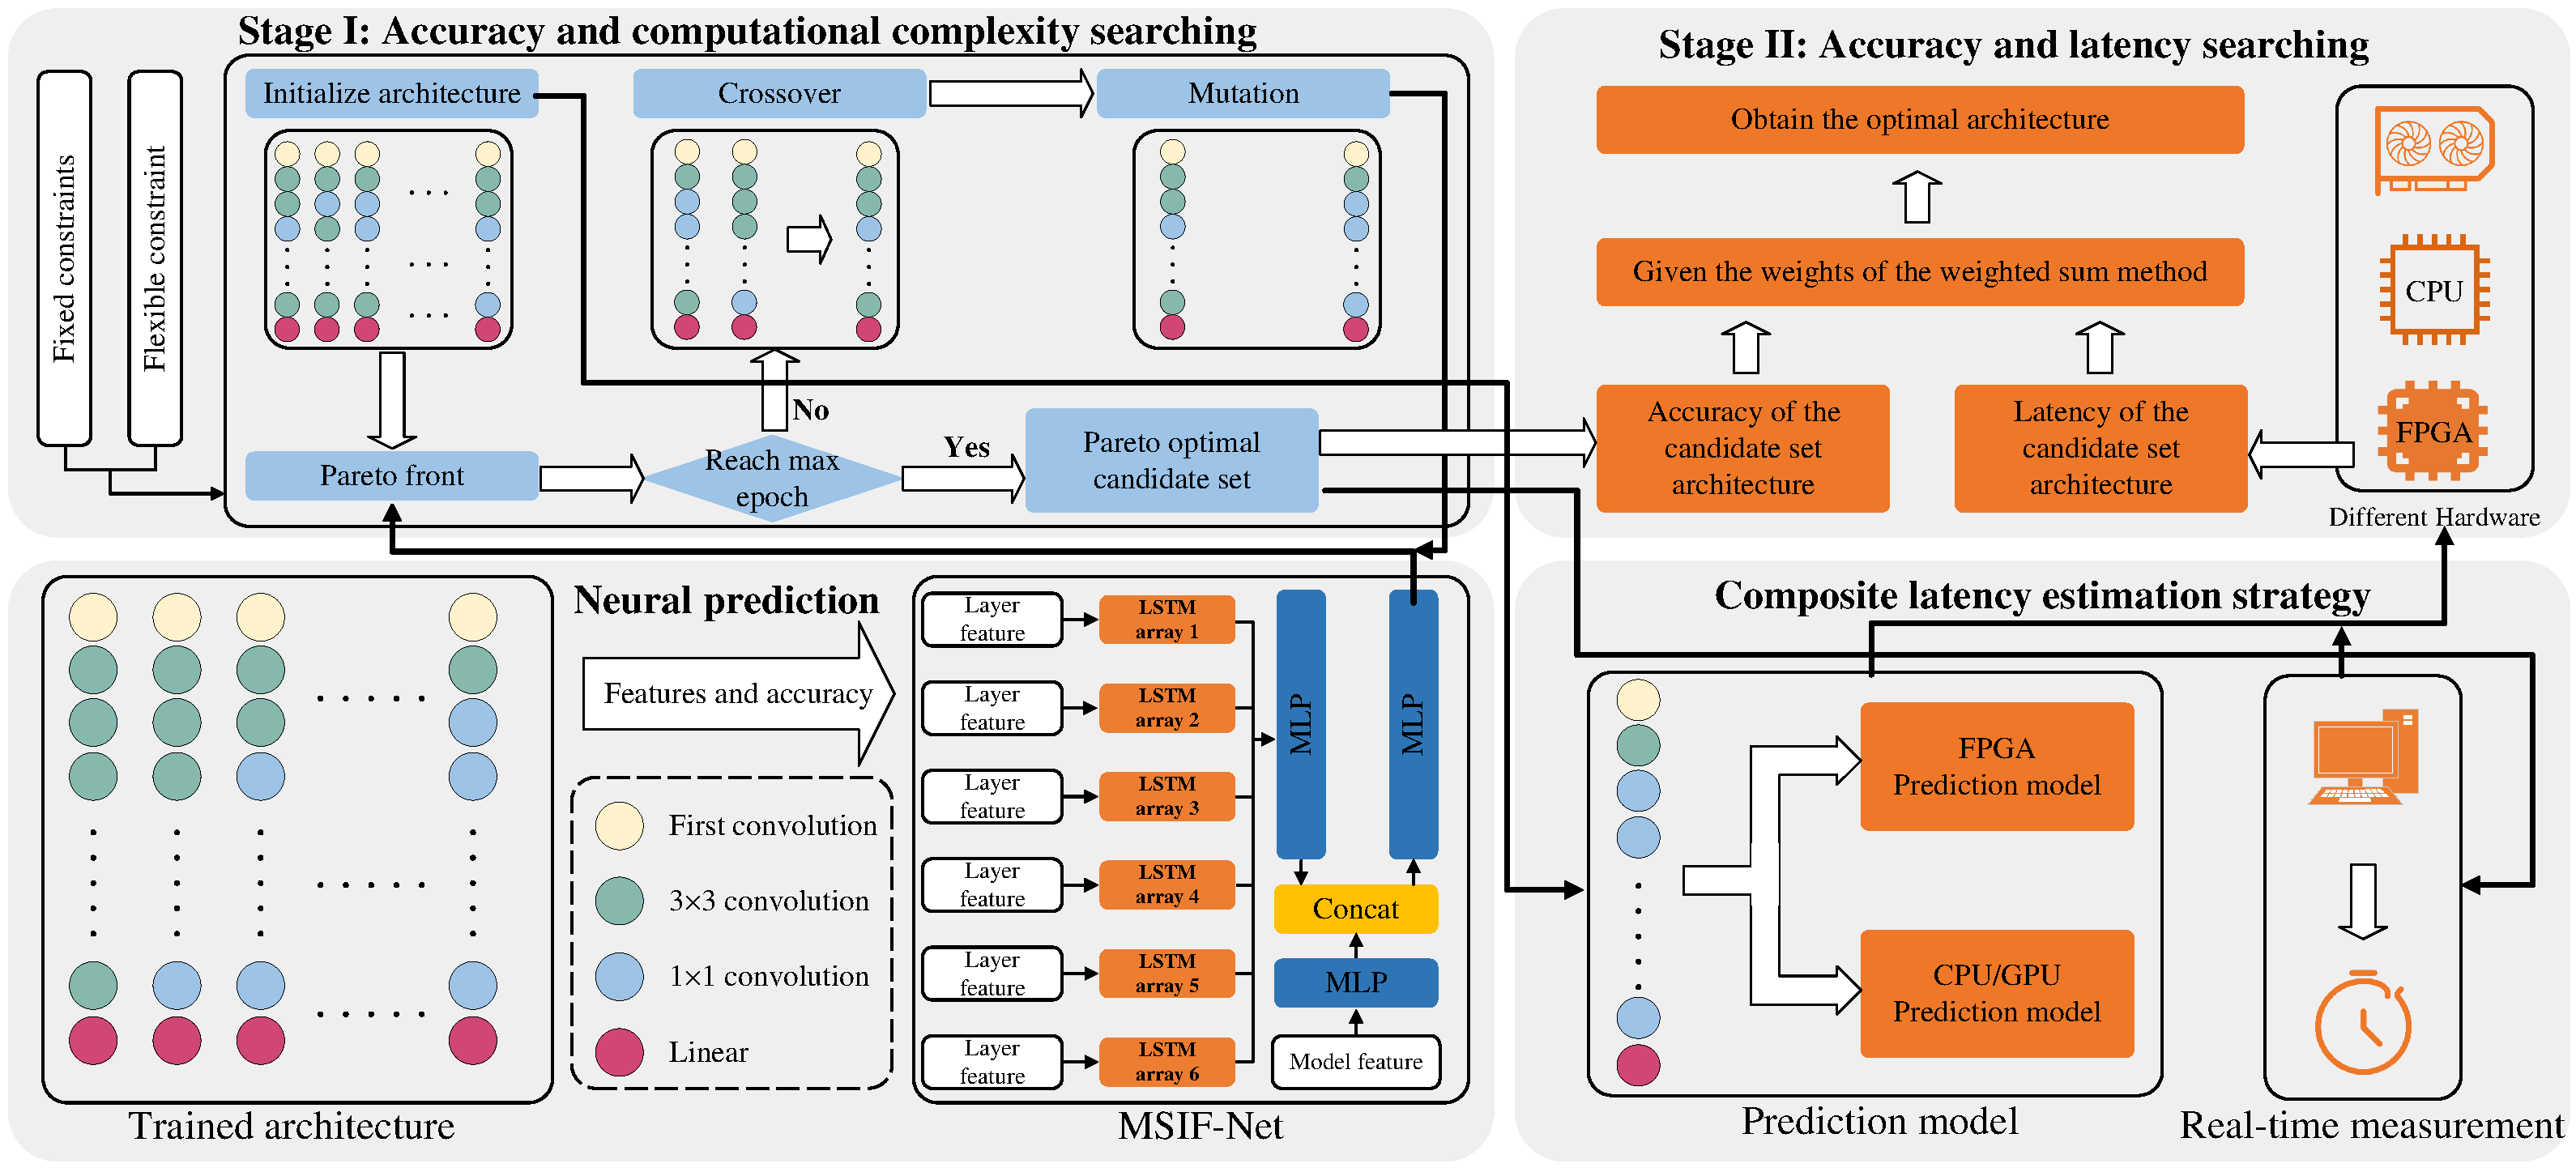
\includegraphics[width=\textwidth]{figs/Figure_3.pdf}
\end{graphicalabstract}

\begin{highlights}
\item Chain-structured BNN NAS for efficient visual recognition across platforms.
\item A two-stage search with CIF-Net accelerate architecture search.
\item Cross-platform latency estimation bridges the gap between OPs and real runtime.
\item Image classification benchmarks show strong accuracy-latency trade-offs.
\end{highlights}

\begin{keywords}
binary neural network \sep 
neural architecture search \sep 
image classification \sep 
diverse hardware platforms \sep 
\end{keywords}

\maketitle

%%========= Introduction
\section{Introduction}
In recent years, binary neural networks (BNNs) have attracted growing attention for efficient visual recognition because they enable fast inference on resource-constrained edge devices. Their advantages have led to applications in image classification~\cite{LIN2025105646, VORABBI2025105524}, object detection~\cite{Lin2025}, and other vision tasks. Existing BNN design mainly follows two paradigms: manual design and neural architecture search (NAS). Manual design methods have progressively narrowed the accuracy gap between BNNs and real-valued networks through improved quantization schemes~\cite{Rastegari2016, Adrian2019,qin2020forward,lin2020rotated,xu2021recu,Tu2022}, better architectures~\cite{Liu2018, Liu2020,Joseph2020,Tu2022,Zhang2022, Guo2022,lee2023insta,Zhang2025}, and optimized training strategies~\cite{Liu2018,martinez2020training,Liu2020,shang2022lipschitz,livochka2021initialization,liu2021adam}.

NAS for BNNs mainly falls into two paradigms: cell-based and chain-structured. \textcolor{red}{Their search-space structures are illustrated in Fig.~\ref{fig:1}(a).} Cell-based NAS (e.g., BATS~\cite{Bulat2020}, BNAS~\cite{Kim2020}, and EBNAS~\cite{Shi2023}) searches for a compact computational cell and stacks it to form the final network. This paradigm enables efficient gradient-based optimization and achieves competitive performance on small-scale datasets such as CIFAR-10/100~\cite{Krizhevsky2009}. However, its search space mainly captures micro-level operator combinations and intra-cell connections. As a result, it is less effective at optimizing macro-level factors such as depth, width allocation, and stage ratios, which are critical for scaling to large benchmarks like ImageNet. In contrast, chain-structured NAS directly searches macro architectures, such as depth, width, and kernel configurations. For example, NAS-BNN~\cite{Lin2025} introduces a training strategy tailored to chain-structured BNN search and achieves slightly higher accuracy than strong handcrafted baselines under the same operation budget on ImageNet. However, existing methods still face two key limitations for real-world deployment: repeated search across platforms is prohibitively expensive, and architecture optimization is often guided by proxy costs (e.g., OPs/FLOPs) rather than measured real-device latency.

\begin{figure}
    \centering
    \begin{tabular}{cc}
        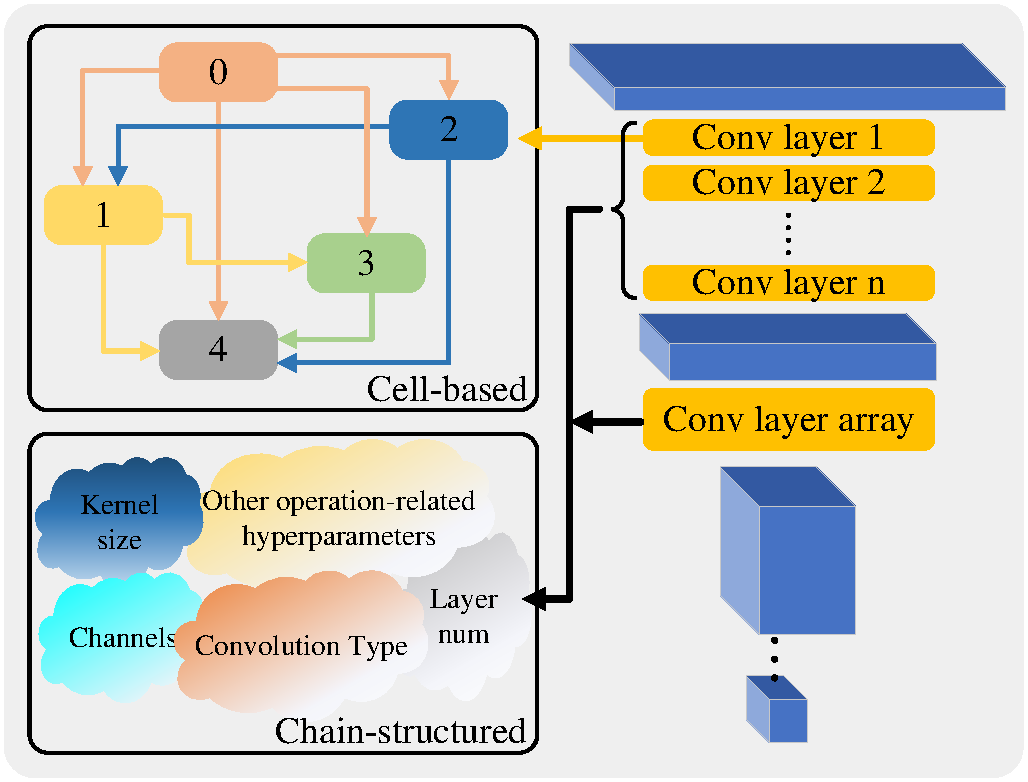
\includegraphics[height=0.20\textheight]{./figs/Figure_1_a.pdf} & 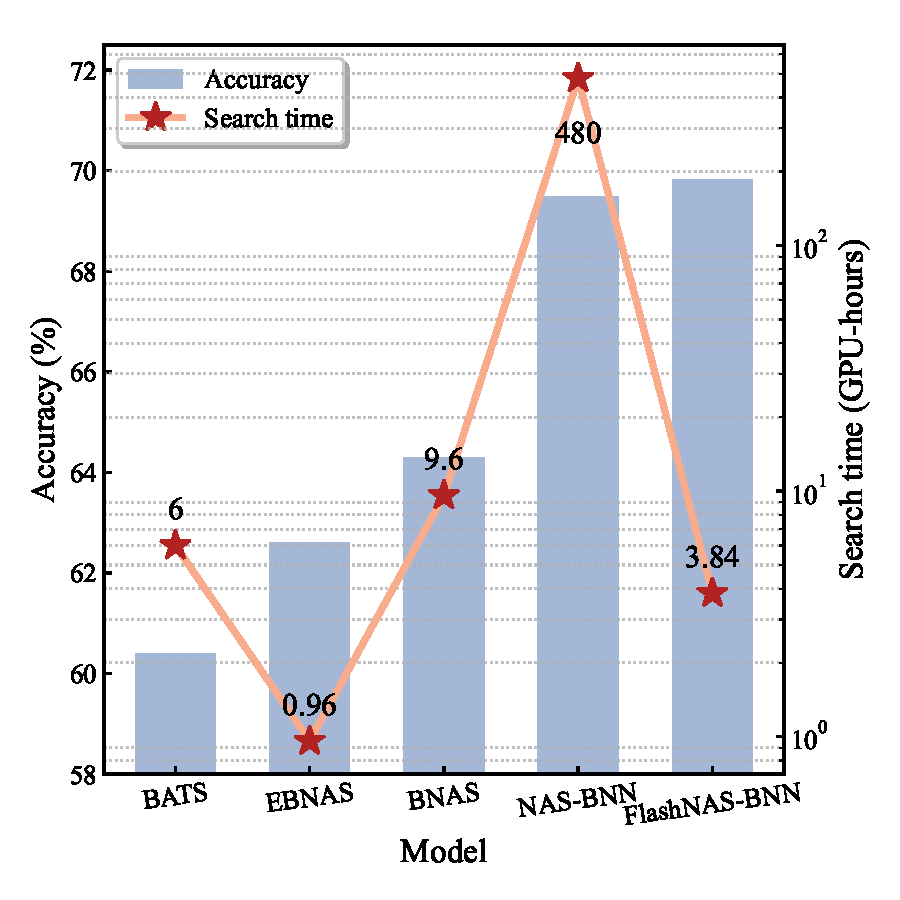
\includegraphics[height=0.20\textheight]{./figs/Figure_1_b.pdf} \\
        \scriptsize (a) & \scriptsize (b)\\
    \end{tabular}
    \caption{\textcolor{red}{Comparison of cell-based and chain-structured NAS. (a) Search-space illustration. (b) Reported ImageNet-1K Top-1 accuracy and average search cost for three platforms. Training schedules are listed in Table~\ref{tab:3}; costs follow Table~\ref{tab:search_cost}, including offline preparation for FlashNAS-BNN.}}\label{fig:1}
\end{figure}

\textcolor{red}{Chain-structured NAS can incur high search costs when each target platform requires an independent search. NAS-BNN reports a search cost of 480 GPU-hours per platform, totaling 1440 GPU-hours for three independent searches. This motivates reuse across platforms. Figure~\ref{fig:1}(b) summarizes the reported accuracy and the average search cost per platform for three target platforms. FlashNAS-BNN-E achieves 69.82\% Top-1 accuracy, compared with 60.4\%, 62.6\%, and 64.3\% for BATS, EBNAS, and BNAS, respectively, under their reported training protocols. With the same predictor and Stage-I candidates reused, FlashNAS-BNN incurs 1365.17 GPU-hours over three platforms, or 455.06 GPU-hours per platform, versus 480 GPU-hours for NAS-BNN under the accounting in Table~\ref{tab:search_cost}. The cost advantage arises from reuse across multiple platforms (Section~\ref{sec:search_time}).}

Second, prior BNN NAS designs often rely on OPs/FLOPs as the primary latency proxy, implicitly assuming a strong monotonic relation between OPs and runtime and thus understating the effect of architectural choices on real-device latency. As shown in Fig.~\ref{fig:2}(a), NAS-BNN has lower OPs than BNAS but higher measured latency on Cortex-X4 with Huawei's Noah's Bolt toolkit~\cite{Huawei2020}. To investigate this mismatch, we retrain NAS-BNN with the same training recipe and analyze two representative architectures. Fig.~\ref{fig:2}(b) shows that although Arch~2 has higher cumulative OPs, its cumulative latency grows more slowly in later layers, resulting in lower end-to-end runtime.

\begin{figure}
    \centering
    \begin{tabular}{cc}
        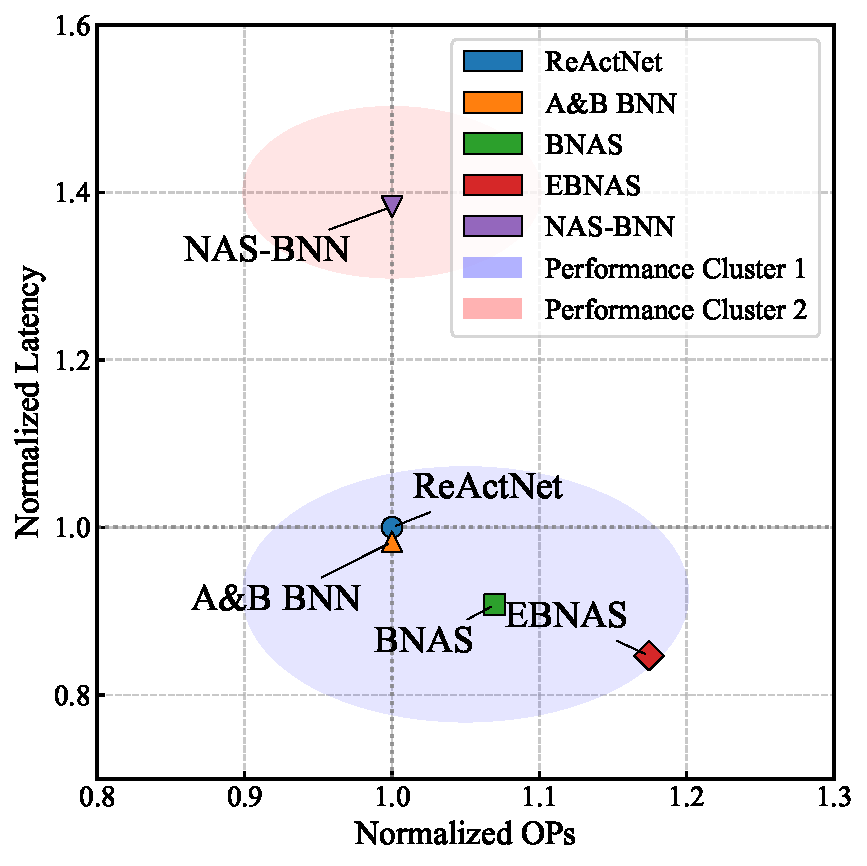
\includegraphics[height=1.8in]{./figs/Figure_2_a.pdf} & 
        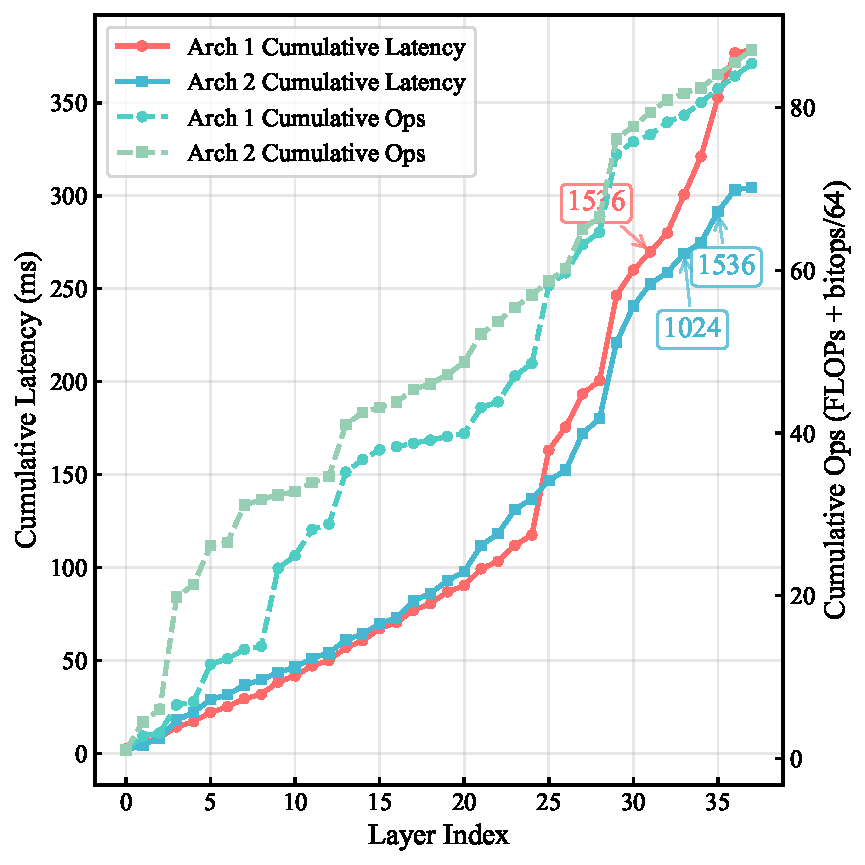
\includegraphics[height=1.8in]{./figs/Figure_2_b.pdf} \\ [-0.5pt]
        \scriptsize (a)  & 
        \scriptsize (b) 
    \end{tabular}
    \caption{OPs are an unreliable proxy for real-device latency. (a) Normalized latency--OP comparison on Cortex-X4 for representative BNNs on ImageNet-100, with both axes normalized to ReActNet (OP/OP$_{\text{ReActNet}}$ and Lat/Lat$_{\text{ReActNet}}$). (b) Controlled case study of two NAS-BNN architectures: cumulative measured latency versus cumulative OPs along network depth shows that a model with higher OPs can still achieve lower end-to-end latency. Labels denote channel numbers.}\label{fig:2}
\end{figure}

In view of the above challenges, this paper proposes FlashNAS-BNN, an efficient chain-structured binary NAS framework for cross-platform visual recognition. Specifically, FlashNAS-BNN improves efficiency in two complementary aspects: search efficiency and deployment efficiency. For search efficiency, we introduce a chain information flow network (CIF-Net) to predict candidate accuracy, \textcolor{red}{avoiding per-candidate sub-network training during search and thereby accelerating candidate evaluation} \textbf{(Solve problem 1)}. We further adopt a two-stage strategy that \textcolor{red}{first screens candidates by predicted accuracy and then evaluates platform-specific latency for the retained architectures. The screened set is reused across platforms to reduce repeated search effort} \textbf{(Solve problem 1)}. For deployment efficiency, we introduce cross-platform latency estimation (CLE), which selects suitable prediction models according to hardware characteristics to support latency-aware architecture selection \textbf{(Solve problem 2)}. Our main contributions are summarized as follows.

\begin{enumerate}
    \item {\textcolor{red}{FlashNAS-BNN trains a CIF-Net predictor using accuracy labels from sampled sub-networks. CIF-Net then predicts candidate accuracy during search, avoiding candidate-by-candidate sub-network training and substantially reducing online search time. A two-stage strategy screens candidates by predicted accuracy before platform-specific latency evaluation and reuses the screened set across platforms.}}
    \item {CLE targets cross-platform latency optimization by bridging the gap between theoretical OPs and real-world runtime. It utilizes measurable latency proxies and device-specific modeling to provide robust latency estimates for architecture selection across diverse hardware.}
    \item {Experimental results demonstrate that FlashNAS-BNN optimizes latency across CPU, GPU, and FPGA. It outperforms handcrafted (e.g., ReActNet-A) and NAS baselines (e.g., NAS-BNN) by reducing latency by up to 47.1\% over ReActNet-A and \textcolor{red}{by 39.6\% over CPU-targeted NAS-BNN with CLE, at comparable accuracy}. \textcolor{red}{The results demonstrate the effectiveness of the proposed framework for latency-aware BNN search across heterogeneous platforms.}}
\end{enumerate}

%%========= Related Work
\section{Related Work}
\subsection{Neural architecture search for BNNs}
NAS methods based on the cell search space have attracted extensive attention due to their short search times. Typical methods such as BNAS~\cite{Kim2020}, BATS~\cite{Bulat2020} and EBNAS~\cite{Shi2023} require search \textcolor{red}{times of only 9.6, 6 and 0.96 GPU-hours}, respectively. These methods focus the core of the search on the computational cell. But they do not consider the number of neural network layers and the changes in the model's different stage ratios, which leads to poor performance on complex datasets. \textcolor{red}{BNAS, a representative cell-based NAS method, achieves 64.3\% Top-1 accuracy on ImageNet-1000, which cannot reach the accuracy of the original ReActNet-A.}

NAS methods relying on chain-structured search spaces have demonstrated accuracy improvements on complex datasets. For instance, NAS-BNN~\cite{Lin2025} attains 0.1\% higher accuracy than ReActNet-A under equivalent computational budgets. However, these approaches still face practical deployment challenges due to their computationally intensive search processes. Specifically, NAS-BNN requires 480 GPU-hours respectively, severely limiting scalability.

Despite the accuracy improvements in chain-structured NAS, the lengthy search time associated with these methods has driven us to explore ways to accelerate the search.

\subsection{Performance prediction techniques}
Performance prediction techniques, encompassing both accuracy and latency estimation, have primarily focused on cell-based NAS. For accuracy, methods range from feature-based regressors (e.g., $\nu$-SVR~\cite{Baker2017}) to learned encoders such as LSTM/MLP (Peephole~\cite{Deng2017}) and GNNs~\cite{Qin2022,Wen2020}. Similarly, recent latency predictors like BRP-NAS and CLCDLP employ graph-based models to capture cell topology. However, these approaches rely heavily on cell-level encodings, making them ill-suited for chain-structured architectures where macro-level configurations (e.g., depth and width schedules) dominate performance. Furthermore, topology-centric latency predictors often under-emphasize measurable hardware constraints; for instance, BRP-NAS neglects measurable latency-driving factors, while CLCDLP's latency feature branch is often overshadowed by its graph encoding. \textcolor{red}{nn-Meter~\cite{Zhang2021nnMeter} captures backend operator fusion and estimates model latency by summing kernel-level random-forest predictions. Its additive formulation assumes sequential kernel execution and does not directly represent overlapping FPGA pipeline stages. Motivated by this execution-model difference, CLE combines measurable computation and data-movement proxies with platform-specific estimators: sequence regression for FPGA and additive estimation for non-overlapped CPU/GPU execution.}

%%========= Method
\begin{figure}
    \centering
    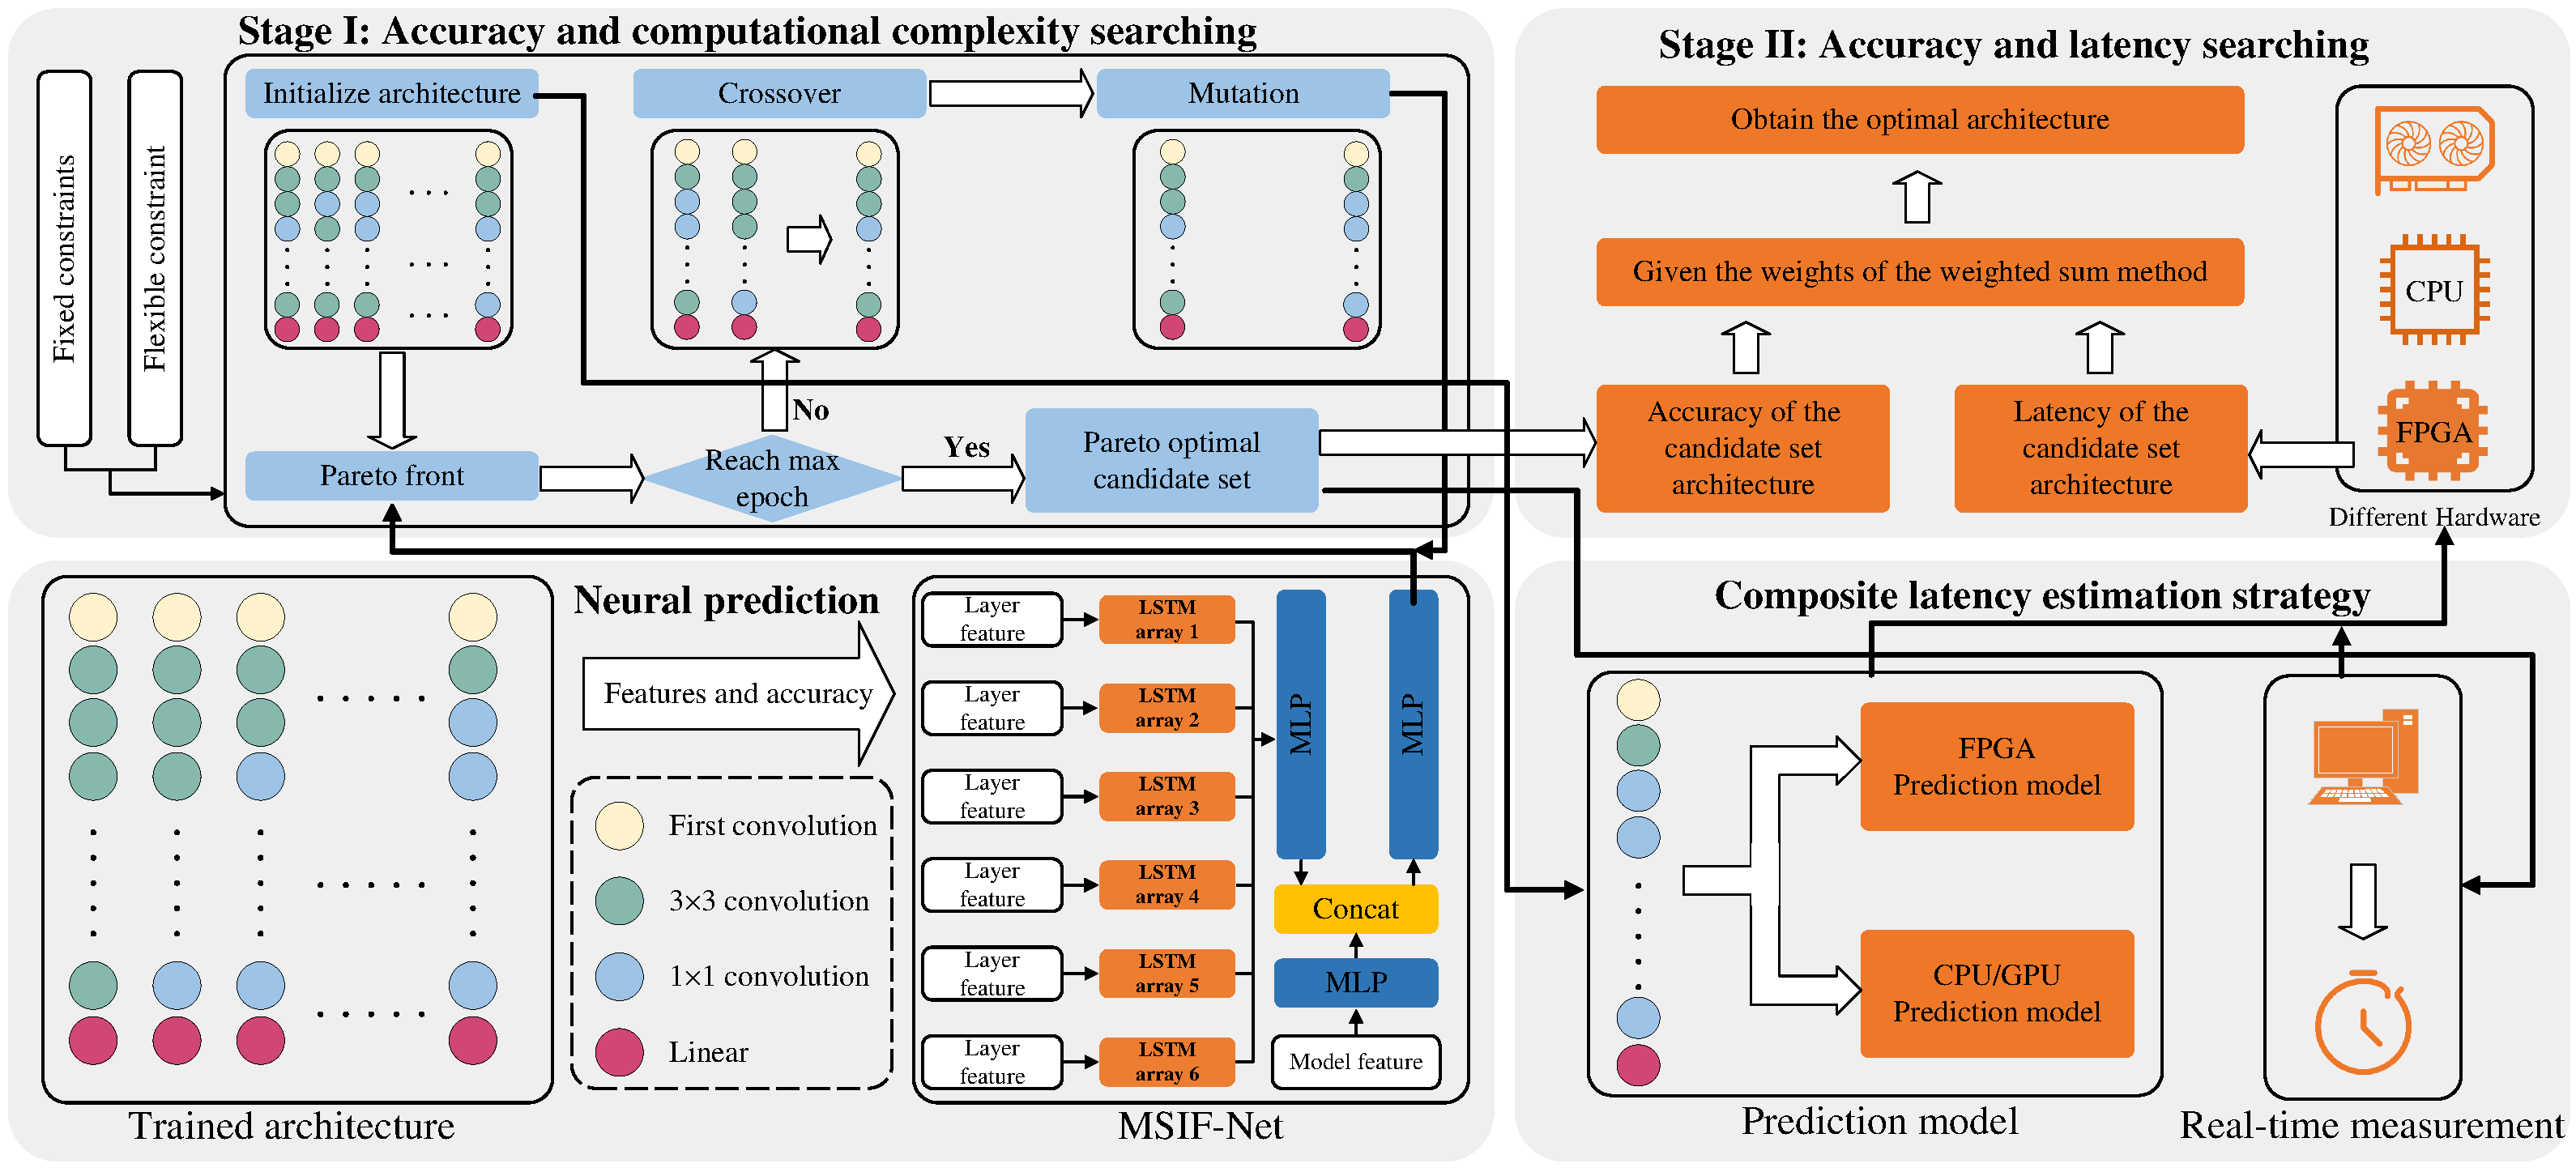
\includegraphics[width=0.8\columnwidth]{./figs/Figure_3.pdf}
    \caption{FlashNAS-BNN search framework. The first stage performs accuracy-OPs exploration using CIF-Net to rapidly evaluate candidate architectures. The second stage refines the candidate set for a target platform using cross-platform latency estimation and a weighted objective to obtain the final latency-optimized architecture.}\label{fig:3}
\end{figure}
\section{Method}
This section presents FlashNAS-BNN, an efficient chain-structured binary NAS framework. It improves search efficiency via CIF-Net and a two-stage strategy that decouples accuracy exploration from latency optimization, and improves deployment efficiency via CLE for robust cross-platform latency estimation and latency-aware architecture selection (Fig.~\ref{fig:3}).

\begin{figure}
    \centering
    \begin{tabular}{cc}
        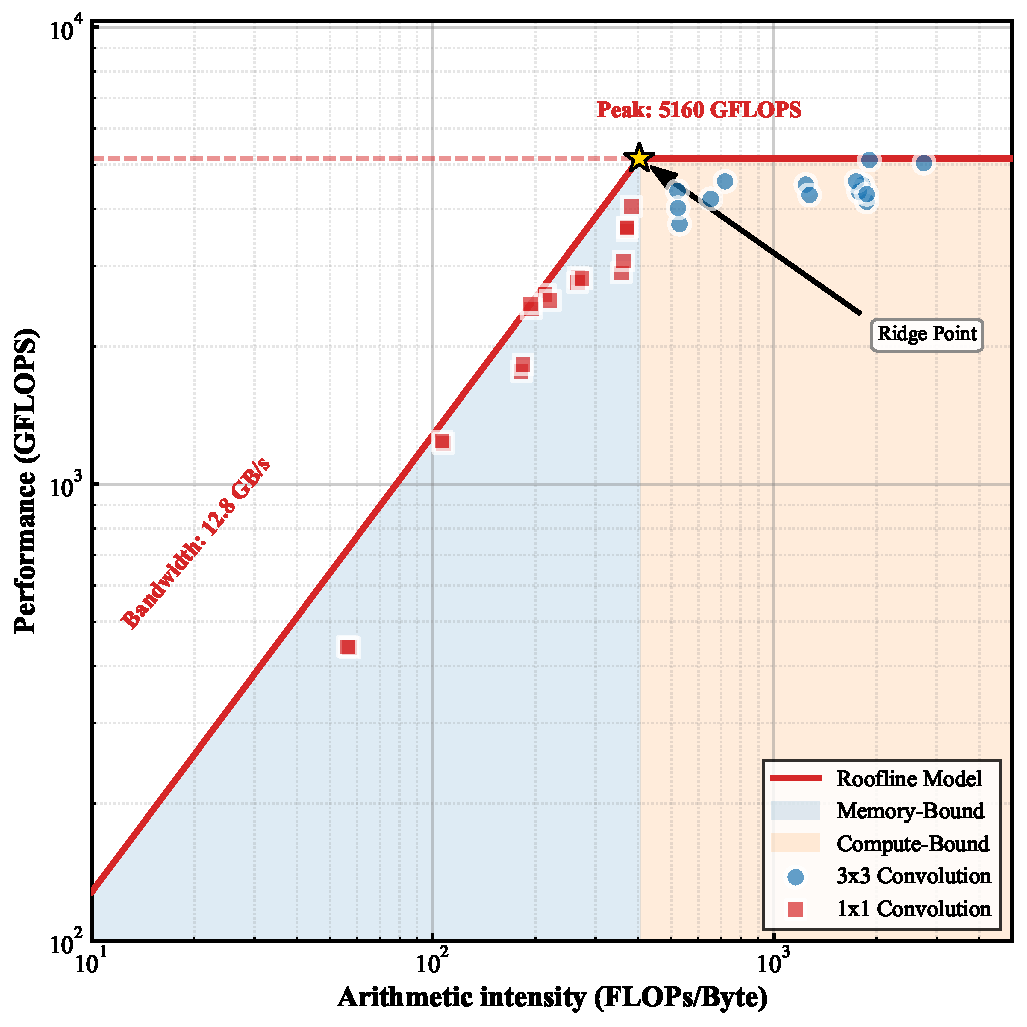
\includegraphics[height=1.7in]{./figs/Figure_4_a.pdf} & 
        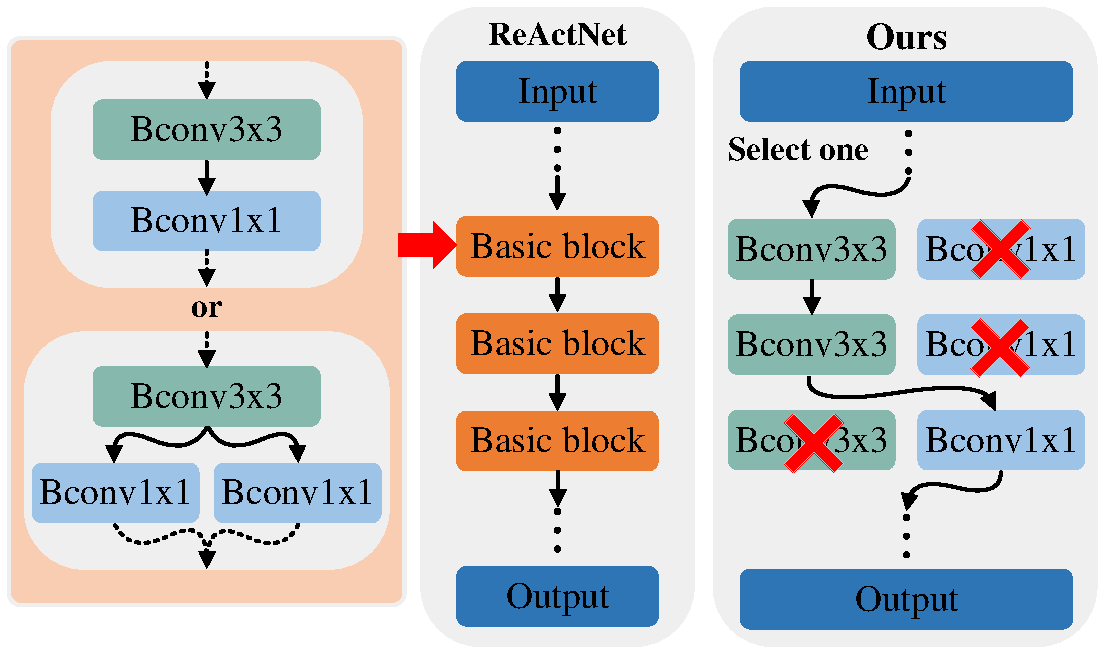
\includegraphics[height=1.7in]{./figs/Figure_4_b.pdf} \\ [-0.5pt]
        \scriptsize (a)  & 
        \scriptsize (b) 
    % \end{tabularx}
    \end{tabular}
    \caption{Roofline analysis and architecture search space. (a) Roofline analysis of ReActNet-style convolutions on FPGA. (b) Searchable depth, width, and kernel configurations beyond the fixed ``3$\times$3 + 1$\times$1'' pattern.}\label{fig:4}
\end{figure}
\begin{table}[ht]
	\centering
	\caption{The Search Space of FlashNAS-BNN. Among them, "Depth", "Channel", and "Kernel" respectively denote depth configurations, channel widths, and kernel sizes.}
	\label{tab:1}
	\small
	\begin{tabular}{c|c|c|c|c}
	\toprule[1.5pt]
	Input & Depth & Channel & Kernel & \makecell{Model\\stage} \\ [0.5ex]
	\midrule
	224$\times$224 & 1 & same with next layer  & 3   & - \\
	112$\times$112 & [1,10] & \{16,24,32,48,64\} & \{1,3\} & 1 \\
	112$\times$112 & [1,10] & \{32,48,64,96,128\}  & \{1,3\} & 2 \\
	56$\times$56 & [1,10] & \{64,96,128,160,192\}  & \{1,3\} & 3 \\
	28$\times$28 & [1,20] & \{160,192,256,320,384\}  & \{1,3\} & 4 \\
	14$\times$14 & [1,20] & \{320,384,512,640,768\}  & \{1,3\} & 5 \\
	7$\times$7 & [1,20] & \{640,768,1024,1280,1536\}  & \{1,3\} & 6 \\
	1$\times$1 & 1 & class  & - & - \\
	\bottomrule[1.5pt]
	\end{tabular}
\end{table}

\subsection{Architecture search space}\label{search_space}
To avoid searching the intractable full BNN design space, we adopt the widely used ReActNet as the backbone template. We fix the overall topology and focus on macro configurations that critically affect real-device latency.

The roofline model motivates considering both computation and data movement, rather than operation count alone. The attained performance on a platform $p$ is bounded by
\begin{equation}
P_{\mathrm{attained}}(p) \leq \min\!\big(\mathrm{Th}_{\max}(p),~\mathrm{BW}(p)I_{\mathrm{device}}(p)\big),
\end{equation}
where $\mathrm{Th}_{\max}(p)$ is the peak compute throughput, $\mathrm{BW}(p)$ is the bandwidth of the memory interface under consideration, and $I_{\mathrm{device}}(p)$ is the operation count divided by the bytes transferred across that interface. The bound uses consistent operation and byte units.

For a standard dense convolution with equal input and output spatial dimensions and equal storage cost per tensor element, we use the following structural intensity proxy, counting one multiply--accumulate as one structural operation:
\begin{equation}
I_{\mathrm{struct}} \approx
\frac{HW C_{\mathrm{in}}C_{\mathrm{out}}K^2}
{HW(C_{\mathrm{in}}+C_{\mathrm{out}})+C_{\mathrm{in}}C_{\mathrm{out}}K^2}.
\label{eq:intensity}
\end{equation}
Further derivations and byte-aware formulations for unequal spatial dimensions are provided in the supplementary material, ``Structural intensity assumptions.''

Eq.~\ref{eq:intensity} shows how channel width and kernel size jointly affect computation and data-movement requirements, motivating their inclusion in the search space. Latency depends on both intensity and the total operation count. Figure~\ref{fig:4}(a) illustrates this computation--data-movement trade-off on FPGA. Stage depth is included separately because it changes the total workload and execution dependencies; its latency effect depends on the deployment schedule, particularly for streaming FPGA implementations. We therefore search depth, width, and kernel configurations, while CLE and measured hardware latency guide platform-specific selection.

The resulting search space is formally parameterized as:
\begin{align}
\text{stage}_i =
\left\{
\text{In}_i, D_i, C_i, K_i
~\Big|~
\text{In}_i = \frac{224}{2^{\max(1,i-1)}},~
D_i\in\mathcal{D}_i,~
C_i\in\mathcal{C}_i,~
K_i\in\mathcal{K}_i
\right\},
\label{eq:define_stage}
\end{align}
Here, $D_i$, $C_i$, and $K_i$ denote the depth, channel width, and kernel size of stage $i$, respectively; their candidate sets are summarized in Table~\ref{tab:1}. Within a fixed-width stage, convolutions use $C_{\mathrm{in}}=C_{\mathrm{out}}=C_i$, while channel-changing transitions retain distinct input and output widths in Eq.~\ref{eq:intensity}.

\subsection{Two-stage search}\label{sec:two_stage}
Let $\mathcal{A}$ denote the chain-structured BNN search space and $\mathcal{P}=\{p_1,\dots,p_M\}$ the target platforms. For architecture $a\in\mathcal{A}$, let $Acc(a)$ denote validation accuracy and $T(a,p)$ the measured end-to-end latency on platform $p\in\mathcal{P}$. For each platform $p$, the goal is to obtain architectures with a favorable accuracy--latency trade-off:
\begin{align}
\min_{a\in\mathcal{A}}~F(a;p)=\big(-Acc(a),~T(a,p)\big).
\label{eq:mo_true}
\end{align}

Directly training the large number of architectures generated during the evolutionary search to obtain $Acc(a)$, and measuring $T(a,p)$ on every platform, is prohibitively expensive. To make the search practical, we introduce two lightweight surrogates: an accuracy predictor $\widehat{Acc}(a)$ (CIF-Net) and a latency estimator $\hat{T}(a,p)$ (CLE), which jointly drive a two-stage procedure, as summarized in supplementary material 2. Specifically, we decouple the optimization into a platform-agnostic exploration stage that screens architectures using $\widehat{Acc}(a)$, and a platform-specific stage in which CLE provides $\hat{T}(a,p)$ for latency-aware evaluation and selection on each target platform.

In the first stage, \textcolor{red}{we perform platform-agnostic exploration over} $\mathcal{A}$ to derive a reusable candidate set $\mathcal{A}_{\text{opt}}$. The exploration is guided by predicted accuracy $\widehat{Acc}(a)$ from CIF-Net and the platform-independent operation cost $OP(a)$.
We aim to approximate the pareto set under the bi-objective $(-\widehat{Acc}(a),\,OP(a))$:
\begin{align}
\mathcal{A}_{\text{opt}}
=
\operatorname{Pareto}\!\left(
\left\{ (-\widehat{Acc}(a),~ OP(a)) ~\middle|~ a \in \mathcal{A} \right\}
\right).
\label{eq:aopt}
\end{align}
To obtain $\mathcal{A}_{\text{opt}}$ efficiently, we adopt the NAS-BNN pareto-front search strategy~\cite{Lin2025}.

\textcolor{red}{The evolutionary procedure starts from $N_{\text{init}}$ candidate architectures represented by their stage depths, channel widths, and convolution choices in Section~\ref{search_space}. Each iteration generates $N_{\text{cross}}$ crossover offspring by recombining two parents and $N_{\text{mut}}$ mutation offspring by perturbing a parent's architectural choices. Candidate generation respects the search-space structure and the specified OP budget. CIF-Net predicts candidate accuracy without training each candidate network. Non-dominated filtering of parents and offspring under $(-\widehat{Acc},OP)$ retains the accuracy--OPs trade-offs for subsequent exploration. After $iter$ evolutionary updates, the retained candidates form the approximate set $\mathcal{A}_{\text{opt}}$ passed to Stage II.}

\textcolor{red}{In the second stage, we select an architecture for each target platform $p$ from the same candidate set $\mathcal{A}_{\text{opt}}$ using a scalarized objective that combines predicted accuracy and estimated latency.}
We apply min--max normalization over the same candidate set $\mathcal{A}_{\text{opt}}$:
\begin{align}
\tilde{f}_1(a) &= \frac{\widehat{Acc}_{\max}-\widehat{Acc}(a)}{\widehat{Acc}_{\max}-\widehat{Acc}_{\min}+\epsilon},
\label{eq:norm_acc}\\
\tilde{f}_2(a,p) &= \frac{\hat{T}(a,p)-\hat{T}_{\min}(p)}{\hat{T}_{\max}(p)-\hat{T}_{\min}(p)+\epsilon},
\label{eq:norm_lat}
\end{align}
where $\widehat{Acc}_{\max}$ and $\widehat{Acc}_{\min}$ are computed over $\{\widehat{Acc}(a)\}_{a\in\mathcal{A}_{\text{opt}}}$,
and $\hat{T}_{\max}(p)$ and $\hat{T}_{\min}(p)$ are computed over $\{\hat{T}(a,p)\}_{a\in\mathcal{A}_{\text{opt}}}$ for the same platform $p$.
The platform-specific objective is then defined as:
\begin{align}
\min_{a\in\mathcal{A}_{\text{opt}}}~ \tilde{F}(a;p)
= w_{\mathrm{Lat}} \tilde{f}_1(a) + (1-w_{\mathrm{Lat}}) \tilde{f}_2(a,p),
\quad w_{\mathrm{Lat}}\in[0,1],
\label{eq:final_objective}
\end{align}
Here, $w_{\mathrm{Lat}}$ controls the accuracy--latency trade-off: $w_{\mathrm{Lat}}=1$ optimizes accuracy only, while $w_{\mathrm{Lat}}=0$ optimizes latency only. The latency estimate $\hat{T}(a,p)$ is provided by CLE; when real-device evaluation is feasible, we set $\hat{T}(a,p) \leftarrow T(a,p)$ to use measured latency directly.
The constant $\epsilon$ avoids numerical issues when the normalization range is small.

\begin{figure}
    \centering
    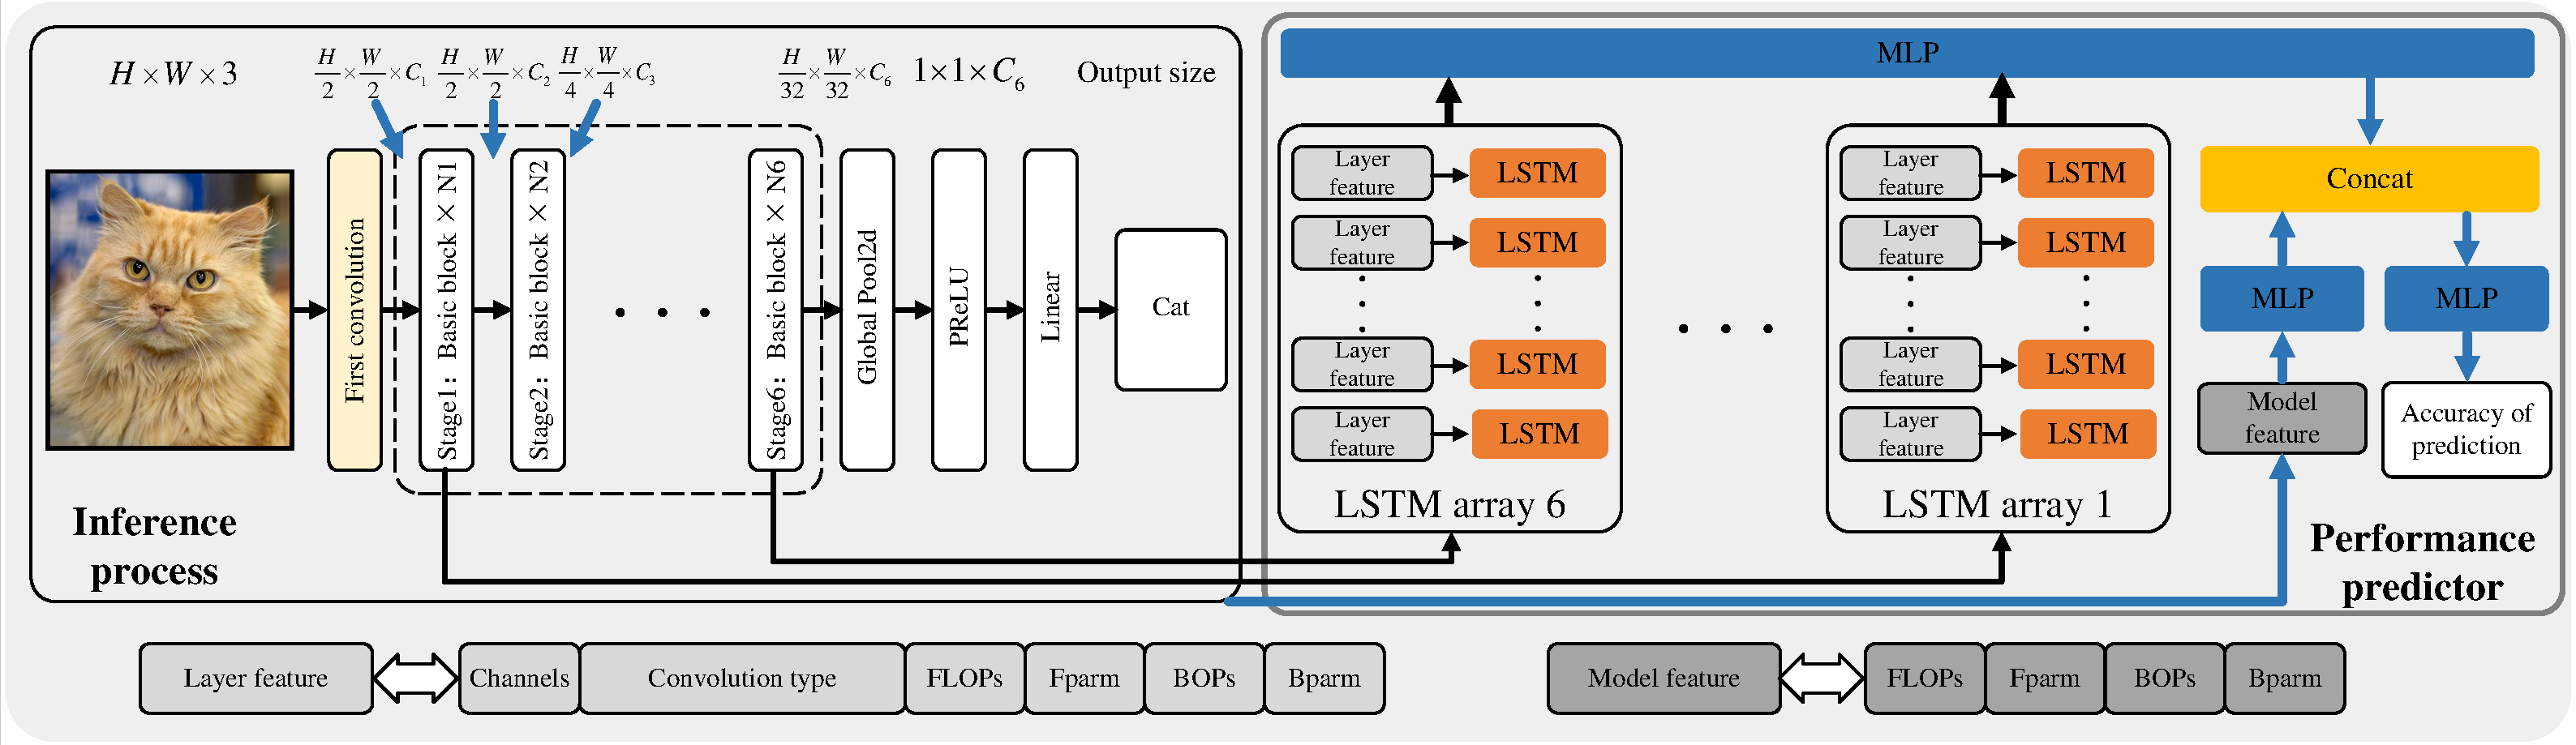
\includegraphics[width=0.8\columnwidth]{./figs/Figure_5.pdf}
    \caption{Accuracy predictor. The chain-structured BNN is decomposed into $S{=}6$ stages. Each stage is encoded as a layer sequence and processed by a dedicated LSTM array to capture inter-layer dependencies.}\label{fig:5}
\end{figure}
\subsection{Chain information flow network}
We first present an architecture encoding scheme for chain-structured BNNs, and then describe CIF-Net for accuracy prediction based on this encoding.

\subsubsection{Architecture encoding scheme}
Following Sec.~\ref{search_space} (Eq.~(\ref{eq:define_stage})), a chain-structured BNN is partitioned into $S$ macro stages, each corresponding to a contiguous block of layers at a fixed activation resolution. We therefore represent an architecture as a stage-wise ordered layer sequence, i.e., $\{ \{ \ell_{s,t} \}_{t=1}^{N_s} \}_{s=1}^{S}$, where $N_s$ is the number of layers in stage $s$.

Each layer is treated as a node and encoded by a multi-attribute feature vector that captures both structural choices and computational characteristics.
Specifically, the node features include: channel width (Channel), convolution type (Conv-type, one-hot), floating-point operations (FLOPs), floating-point parameters (Fparm), binary operations (BOPs), and binary parameters (Bparm).
This layer-wise encoding provides fine-grained cues across stages, enabling the predictor to better model the macro configurations (e.g., depth/width schedules and stage-wise variations) that dominate chain-structured architectures.

Since FLOPs, Fparm, BOPs, and Bparm span several orders of magnitude, we apply a $\log_{10}$ transform to these quantities to compress their dynamic range and improve numerical stability during training.
The resulting stage-wise layer features $\{f_{s,t}(a)\}$ serve as the input to CIF-Net for predicting $\widehat{Acc}(a)$.

\subsubsection{Accuracy predictor network} 
\textcolor{red}{As shown in Fig.~\ref{fig:5}, CIF-Net encodes the layer features $\{f_{s,t}(a)\}$ of each stage using a dedicated LSTM to capture inter-layer dependencies within the same resolution, producing a stage embedding $z_s$.}
The $S$ stage embeddings are then fused by an MLP to obtain a holistic representation of the architecture.
In parallel, we compute a global feature vector $f_g(a)$ that summarizes architecture-level statistics (e.g., total depth, aggregated complexity, and other global descriptors).
Finally, the fused stage representation and the global representation are concatenated and fed into an output MLP to produce the predicted accuracy $\widehat{Acc}(a)$.

Formally, for stage $s\in\{1,\dots,S\}$ with $N_s$ layers, the input feature of the $t$-th layer is denoted by $f_{s,t}(a)\in\mathbb{R}^{d_l}$, where $d_l$ is the layer feature dimension.
The forward computation of CIF-Net is summarized as:
\begin{align}
(h_{s,t},c_{s,t}) &= \mathrm{LSTM}_s\!\left(f_{s,t}(a),~(h_{s,t-1},c_{s,t-1})\right), \quad t=1,\dots,N_s, \label{eq:cif_lstm}\\
z_s &= h_{s,N_s}, \quad s=1,\dots,S, \label{eq:cif_stage}\\
z_l &= \mathrm{MLP}_l\!\left([z_1,\dots,z_S]\right), \label{eq:cif_fuse}\\
z_g &= \mathrm{MLP}_g\!\left(f_g(a)\right), \label{eq:cif_global}\\
\widehat{Acc}(a) &= \mathrm{MLP}_o\!\left([z_l, z_g]\right). \label{eq:cif_out}
\end{align}
Here, $(h_{s,t},c_{s,t})$ are the hidden and cell states of the LSTM for stage $s$, $z_s$ is the stage embedding, $z_l$ aggregates stage-wise information, and $z_g$ encodes global architecture attributes.

\subsection{Cross-platform latency estimation}\label{sec:cle}
\textcolor{red}{CLE estimates platform-specific latency $\hat{T}(a,p)$ from computation and data-movement proxies, including InputSize/OutputSize, Fparm/Bparm, and FLOPs/BOPs. It uses platform-specific estimators:}
\begin{align}
\hat{T}(a,p)=
\begin{cases}
\hat{T}_{\mathrm{FPGA}}(a,p), & \tau(p)=\mathrm{FPGA},\\
\hat{T}_{\mathrm{CG}}(a,p),   & \tau(p)\in\{\mathrm{CPU},\mathrm{GPU}\},
\end{cases}
\label{eq:cle_piecewise}
\end{align}
\textcolor{red}{Here, $p$ denotes the target device and deployment backend, and $\tau(p)$ denotes its device type.}

\begin{figure}
    \centering
    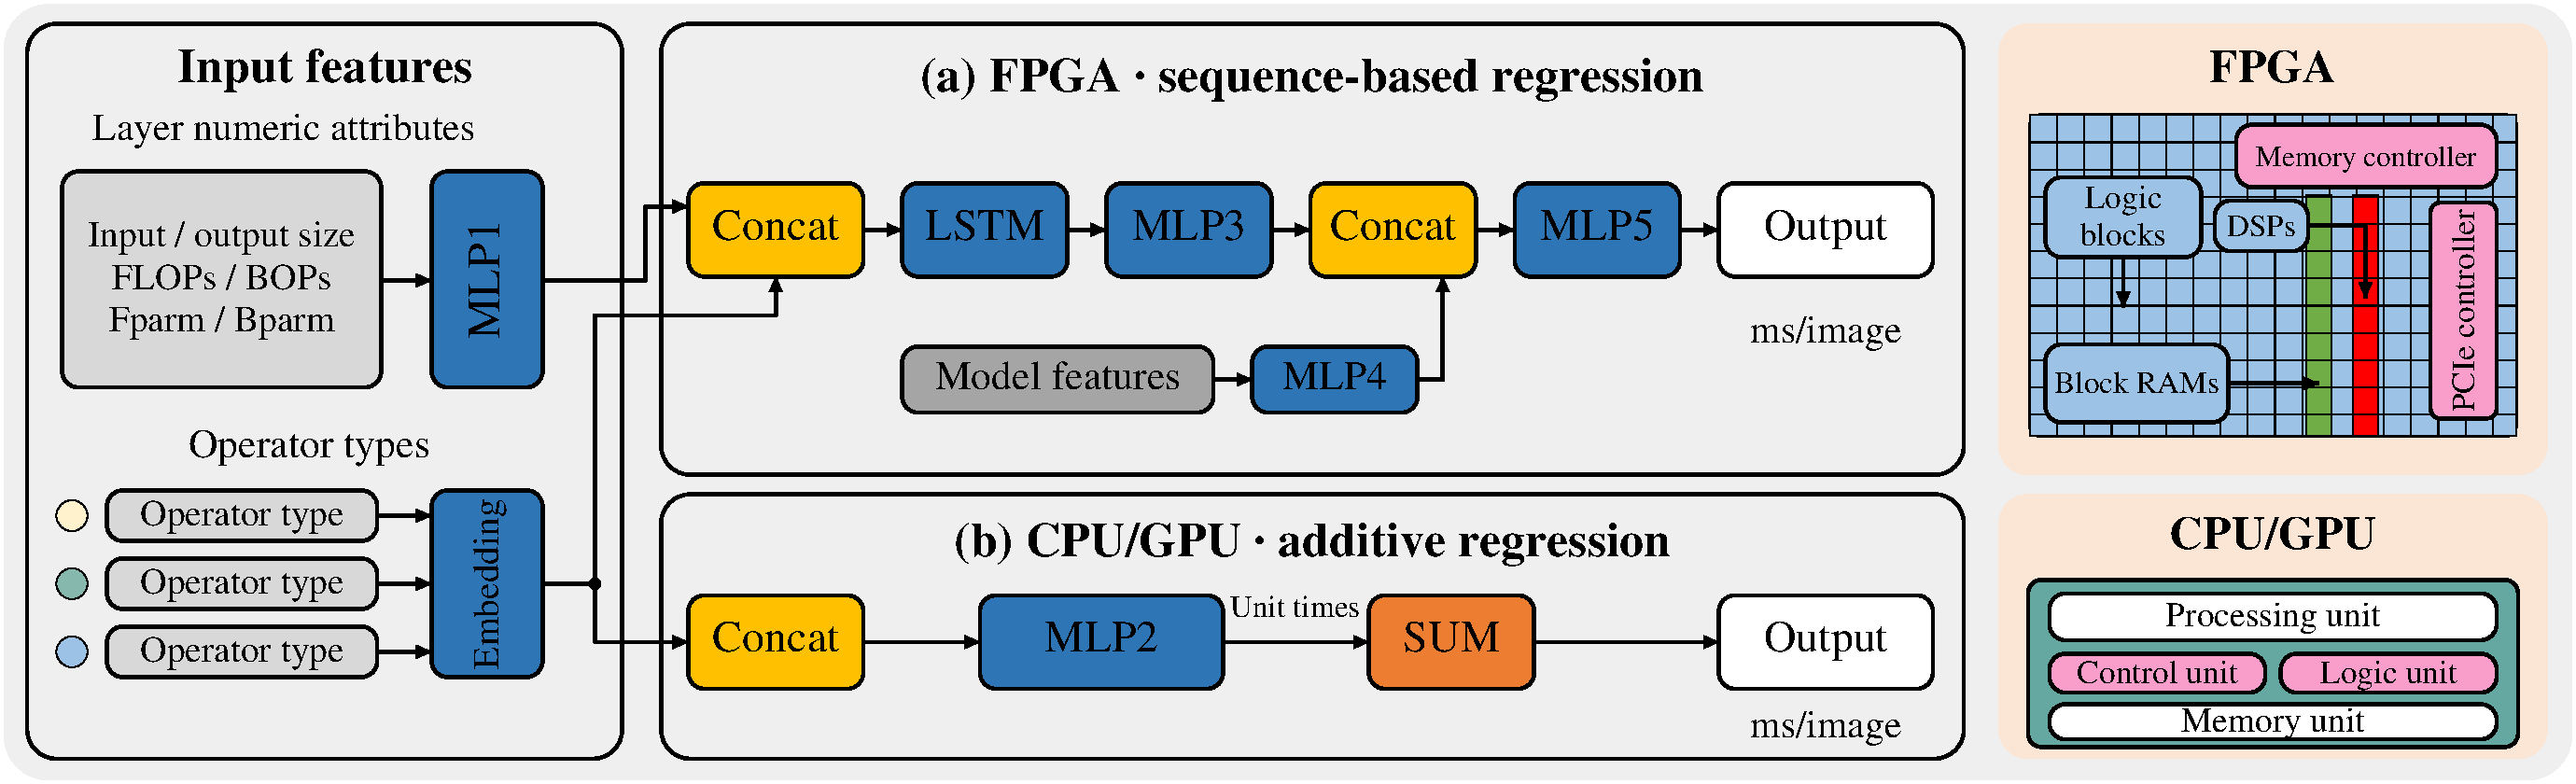
\includegraphics[width=0.8\columnwidth]{figs/Figure_6.pdf}
    \caption{\textcolor{red}{Platform-specific latency prediction models. FPGA uses an LSTM layer-sequence encoder fused with global architecture features to regress end-to-end latency. CPU/GPU use additive execution-unit estimates under non-overlapped scheduling.}}
    \label{fig:6}
\end{figure}

\subsubsection{FPGA}
\textcolor{red}{In the FPGA streaming dataflow, overlapping stages make a sum of independent layer times insufficient to describe end-to-end latency. CLE-FPGA therefore learns latency directly from the layer sequence and global architecture features.}

\textcolor{red}{Let $t_i$ denote the operator type and $x_i(a)$ contain numeric layer attributes, including channel widths, kernel size, activation sizes, and complexity terms. CLE-FPGA encodes the ordered layer sequence and fuses it with global architecture features $f_g(a)$:}
\begin{align}
f^{(i)}_{\mathrm{layer}}(a) &= \big[\mathrm{Emb}(t_i),~\mathrm{MLP}_1(x_i(a))\big], \label{eq:fpga_layer_feat}\\
f_{\mathrm{seq}}(a) &= \mathrm{MLP}_3\!\left(\mathrm{LSTM}\!\left(\{f^{(i)}_{\mathrm{layer}}(a)\}_{i=1}^{m(a)}\right)\right), \\
\hat{T}_{\mathrm{FPGA}}(a,p) &= \mathrm{MLP}_5\!\left(\big[\mathrm{MLP}_4(f_g(a)),~f_{\mathrm{seq}}(a)\big]\right).
\label{eq:fpga_sequence_hat}
\end{align}
\textcolor{red}{The sequence encoder represents stage order and neighboring layer configurations, while the global branch summarizes architecture-level computation and data movement. The fused regressor is trained on measured end-to-end latency.}

\subsubsection{CPU and GPU}
\textcolor{red}{For the non-overlapped CPU/GPU execution considered here, CLE sums predicted execution-unit latencies, treating fused operators as a single unit. With $q(a,p)$ units and features $f^{(j)}_{\mathrm{unit}}(a,p)=[\mathrm{Emb}(t_j),x_j(a,p)]$, we use}
\begin{align}
\hat{T}^{(j)}_{\mathrm{unit}}(a,p) &= \mathrm{MLP}_{2,p}\!\left(f^{(j)}_{\mathrm{unit}}(a,p)\right), \label{eq:cpugpu_unit_hat}\\
\hat{T}_{\mathrm{CG}}(a,p) &= \sum_{j=1}^{q(a,p)}\hat{T}^{(j)}_{\mathrm{unit}}(a,p).
\label{eq:cpugpu_hat}
\end{align}


%%========= Experimental setup
\section{Experimental setup}
\subsection{Dataset}
\textcolor{red}{We evaluate on ImageNet-1000~\cite{Deng2009}, ImageNet-100, and CIFAR-10/100~\cite{Krizhevsky2009}.} ImageNet-1000 contains 1.28M training and 50K validation images at 224$\times$224 resolution. ImageNet-100 is a 100-class subset of ImageNet-1000, with 1300 training and 50 validation images per class. CIFAR-10/100 consist of 32$\times$32 color images with 50K training and 10K test samples, containing 10 and 100 classes, respectively.

\subsection{Implementation details}

\subsubsection{Training of accuracy predictor.} 
\textcolor{red}{We train CIF-Net separately for the ImageNet and CIFAR experiments, using 25-epoch accuracy labels from ImageNet-100 and CIFAR-100, respectively. Each predictor uses labels from 750 architectures sampled from the 9--33-layer search space, with 30 architectures per depth. CIF-Net is trained on an 80\%/20\% train/test split using AdamW~\cite{Loshchilov2019} (lr $=10^{-5}$, batch size $=8$) on four NVIDIA RTX 4090 GPUs. Label-generation protocols and predictor reuse are detailed in Supplementary Section 3.}

\subsubsection{Training of latency predictor.} 
We measure end-to-end inference latency on three representative deployment platforms. For the mobile CPU (Cortex-X4) and mobile GPU (Mali-G77), latency is profiled using Huawei's Noah's Bolt toolkit~\cite{Huawei2020}. For FPGA, we implement the accelerator on XC7VX690T with Vitis HLS 2022.1 and Vivado 2022.1. The baselines and FlashNAS-BNN use the same FPGA accelerator implementation. We use 500 latency measurements collected from the first-stage search for model training, with a 50\%/50\% train/test split. For latency-predictor training, the optimizer and learning rate remain unchanged, with the training batch size set to 1. \textcolor{red}{Inference latency is reported in ms/image for batch size 32; the full measurement protocol is given in Supplementary Section 1.}

\subsubsection{Search and final training}
BNAS, EBNAS, and NAS-BNN are trained on ImageNet-100 using their respective codebases and training protocols.
All searches use a single RTX 4090 GPU and an Intel Xeon E5-2678 v3 CPU, with $N_{\text{init}}=512$, $N_{\text{cross}}=N_{\text{mut}}=128$, and \textcolor{red}{20 evolutionary iterations.}
\textcolor{red}{FlashNAS-BNN-A/B/C use $w_{\mathrm{OP}}=0.25/0.50/0.75$, D/E/F use $w_{\mathrm{OP}}=0.50/0.75/1.00$, and G/H/I use $w_{\mathrm{Lat}}=0.5$ for CPU/GPU/FPGA, respectively. A--F are accuracy--OPs reference variants; G/H/I undergo platform-specific Stage-II selection. Further details are provided in the supplementary material.}
\textcolor{red}{ImageNet-100/1000 models use two-phase Adam training~\cite{kingma2015adam} with batch size 256, an initial learning rate of $1.25\times10^{-3}$ per phase, and weight decay of $10^{-5}/0$ for phases 1/2. Each phase lasts 128 epochs; ImageNet-1000 additionally uses 256 epochs per phase for comparisons with manually designed models and NAS-BNN, while the 128-epoch results are compared with cell-based NAS methods.}
\textcolor{red}{CIFAR-10/100 models are trained directly with quantized weights and activations using the same hyperparameters as BATS~\cite{Bulat2020}: Adam, an initial learning rate of $10^{-3}$, batch size 256, 600 epochs, and zero weight decay.}

%%========= Results and discussion
\section{Results and discussion}
\subsection{Results on CIFAR}
\begin{table}[ht]
\centering
\caption{Comparison of different models on CIFAR-10/CIFAR-100 datasets.}
\small
\begin{tabular}{l c c c c c}
\toprule[1.5pt]
\multicolumn{1}{l}{\multirow{2}{*}{Model}}   & \multicolumn{2}{c}{Top-1 (\%)} & \multicolumn{1}{c}{\multirow{2}{*}{\makecell{Param\\(MB)}}} & \multicolumn{1}{c}{\multirow{2}{*}{\makecell{OPs\\($10^8$)}}} & \multicolumn{1}{c}{\multirow{2}{*}{\makecell{Search\\method} }}\\
\cmidrule{2-3}
& C10 & C100 & & & \\
\midrule
ResNet18~\cite{He2016}  & 93.00 & 75.61 & 11.2 & 5.55 & Manual\\
ReActNet-BiR18~\cite{Liu2020}  & 93.01 & 70.72 & 1.6 & 0.17 & Manual\\
A\&B BNN~\cite{Ma2024}   & 92.64 & 70.28  & 1.6 & 0.11 & Manual\\
\midrule
BNAS~\cite{Kim2020}  & 92.70 & - & 5.6 & 0.16 & Cell-based\\
BATS~\cite{Bulat2020}  & 93.70 &  70.30  & 2.8 & -- & Cell-based\\
EBNAS~\cite{Shi2023}  &  94.04 &  72.99  & 3.1 & -- & Cell-based\\
UBNAS~\cite{tan2024universal}  &  93.34 &  -  & 3.6 & -- & Cell-based\\
\midrule
\rowcolor{gray!30}\textbf{FlashNAS-BNN-A*}  & 93.15 &  70.89  & 1.6 & 0.12 & Chain\\
\rowcolor{gray!30}\textbf{FlashNAS-BNN-B*}  & 93.45 & 72.21 & 2.3 & 0.15 & Chain\\
\rowcolor{gray!30}\textbf{FlashNAS-BNN-C*}  & 94.16 & 73.10 & 3.0 & 0.17 & Chain\\
\bottomrule[1.5pt]
\end{tabular}

\label{tab:2}
\end{table}
As shown in Table~\ref{tab:2}, \textcolor{red}{FlashNAS-BNN achieves competitive accuracy--parameter trade-offs relative to existing manually designed and NAS-based BNNs on CIFAR-10/CIFAR-100.} Under the same 1.6\,MB parameter budget, FlashNAS-BNN-A$^{*}$ achieves 93.15\%/70.89\%, outperforming ReActNet-BiR18 (93.01\%/70.72\%) and A\&B BNN (92.64\%/70.28\%). Against gradient-based NAS baselines, FlashNAS-BNN-B$^{*}$ achieves 72.21\% on CIFAR-100 with 2.3\,MB parameters, exceeding BATS (70.30\%, 2.8\,MB) by \textcolor{red}{1.91 percentage points} while using 17.9\% fewer parameters. \textcolor{red}{FlashNAS-BNN-C$^{*}$ achieves accuracy comparable to EBNAS (94.16\%/73.10\% versus 94.04\%/72.99\%) with slightly fewer parameters (3.0 versus 3.1\,MB).} Here, "$^{*}$" denotes models searched from ReActNet-BiR18.


\subsection{Results on ImageNet}
As shown in Table~\ref{tab:3}, FlashNAS-BNN achieves competitive accuracy on ImageNet-1000 under comparable computational budgets. 
Compared with the manually designed ReActNet-A (69.4\% Top-1, 7.4\,MB, 0.87$\times10^8$ OPs), FlashNAS-BNN-D attains 69.50\% Top-1 accuracy with slightly fewer parameters (7.2\,MB) and the same OP count.
Similarly, FlashNAS-BNN-E reaches 69.82\% Top-1 accuracy at the same OPs, with 10.7\,MB parameters. \textcolor{red}{For comparison with cell-based NAS baselines, FlashNAS-BNN-E trained for 128 epochs per phase achieves 68.91\% Top-1 accuracy, exceeding BATS, EBNAS, and BNAS by 8.51, 6.31, and 4.61 percentage points, respectively.}
Against chain-structured EA-based NAS-BNN, FlashNAS-BNN delivers comparable or higher accuracy (69.50\%/69.82\% vs. 69.49\%).

\begin{table}[ht]
\centering
\caption{Classification results of models training on ImageNet-1000. \textcolor{red}{FlashNAS-BNN results with 128 epochs per phase are used for comparisons with cell-based NAS methods; results with 256 epochs per phase are used for comparisons with manually designed models and NAS-BNN.}}
\small
\resizebox{0.8\textwidth}{!}{
\begin{tabular}{l c c c l c}
\toprule[1.5pt]
Model          & \makecell{Top-1\\(\%)} & \makecell{Parameters\\(MB)} & \makecell{OPs\\($10^8$)} & \textcolor{red}{Training epochs} & Search method \\
\midrule
Bi-Real-Net-18~\cite{Liu2018} & 56.4  & 4.2         & 1.63          &  0 / 256 / 0    & \textcolor{red}{Manual}        \\
ReActNet-A~\cite{Liu2020}     & 69.4  & 7.4        & 0.87          &   0 / 256 / 256    & \textcolor{red}{Manual}        \\
ReActNet-B~\cite{Liu2020}     & 70.1  & 14.4       & 1.63          &   0 / 256 / 256    & \textcolor{red}{Manual}        \\
\midrule
BATS~\cite{Bulat2020} & 60.4  & -                 & 0.99          &    75 / 0 / 75     & Cell-based    \\
EBNAS~\cite{Shi2023}  & 62.6  & 4.6               & 1.02          &    50 / 100 / 100    & Cell-based    \\
BNAS~\cite{Kim2020}   & 64.3  & 6.4               & 4.71          &    50 / 0 / 250     & Cell-based    \\
\midrule
NAS-BNN~\cite{Lin2025}      & 69.49 & 10.0      & 0.87          &    512 / 0 / 100       & Chain  \\
\midrule
\rowcolor{gray!30}  & 68.55 & ~    & ~      &   0 / 128 / 128  & ~  \\
\rowcolor{gray!30}\multirow{-2}{*}{\textbf{FlashNAS-BNN-D}} & 69.50 & \multirow{-2}{*}{7.2}           & \multirow{-2}{*}{0.87}          &   0 / 256 / 256  & \multirow{-2}{*}{Chain}  \\
\rowcolor{gray!30}  & 68.91 & ~    & ~     &   0 / 128 / 128  & ~  \\
\rowcolor{gray!30}\multirow{-2}{*}{\textbf{FlashNAS-BNN-E}} & 69.82 & \multirow{-2}{*}{10.7}    &   \multirow{-2}{*}{0.87}          &   0 / 256 / 256  & \multirow{-2}{*}{Chain}  \\
\bottomrule[1.5pt]
\end{tabular}
}

\label{tab:3}
\end{table}

\subsection{Cross-platform results}
\textcolor{red}{Table~\ref{tab:4} compares ImageNet-100 accuracy and latency on Cortex-X4, Mali-G77, and XC7VX690T. NAS-BNN is evaluated without CLE and with CLE targeting each platform; all selected architectures are measured on all three devices.}

\textcolor{red}{FlashNAS-BNN-F is the accuracy-oriented reference; G/H/I target CPU/GPU/FPGA, respectively.}

\textcolor{red}{FlashNAS-BNN-G achieves the lowest CPU latency in the table, 164.57\,ms at 81.40\% Top-1 accuracy. It reduces latency by 47.1\% relative to ReActNet-A (311.20\,ms), 61.8\% relative to NAS-BNN without CLE (430.29\,ms), and 39.6\% relative to CPU-targeted NAS-BNN with CLE (272.40\,ms). On GPU, FlashNAS-BNN-H achieves 48.45\,ms at 81.86\% Top-1 accuracy, reducing latency by 16.0\% relative to ReActNet-A (57.71\,ms) and 10.6\% relative to GPU-targeted NAS-BNN with CLE (54.20\,ms). On FPGA, FlashNAS-BNN-I achieves 2.340\,ms at 81.61\% Top-1 accuracy, reducing latency by 6.8\% relative to ReActNet-A (2.510\,ms) and 8.6\% relative to FPGA-targeted NAS-BNN with CLE (2.560\,ms). These comparisons show improved accuracy--latency trade-offs relative to the corresponding hardware-targeted NAS-BNN baselines. FlashNAS-BNN-F achieves the highest Top-1 accuracy of 82.07\% at $0.86\times10^8$ OPs. Figure~\ref{fig:7}(a) illustrates the CPU accuracy--latency trade-offs of selected representative architectures.}

\textcolor{red}{EBNAS GPU/FPGA latency is N/A because the evaluated backends lack the required group-convolution kernels.} We compute OPs as BOPs/64 + QOPs/8 + FLOPs, and parameter count as Bparm/8 + Qparm + FLparm$\times$4.

\begin{table}[ht]
    \centering
    \caption{Performance comparison on the ImageNet-100 dataset across different platforms.}
    \small
    \setlength{\tabcolsep}{3pt}
    \begin{tabular}{l c c c c c c c}
    \toprule[1.5pt]
    \multicolumn{1}{l}{\multirow{2}{*}{Model}}          & \multirow{2}{*}{\makecell{Top-1\\(\%)}}             & \multirow{2}{*}{\makecell{Param\\(MB)}}          & \multirow{2}{*}{\makecell{OPs\\($10^8$)}} & \multicolumn{3}{c}{Latency (\textcolor{red}{ms/image})} & \multicolumn{1}{c}{\multirow{2}{*}{CLE }} \\
    \cmidrule{5-7}
    \multicolumn{1}{l}{}                                & \multicolumn{1}{c}{}                                & \multicolumn{1}{c}{}                                        & \multicolumn{1}{c}{}                          & CPU      & GPU    & FPGA   & \multicolumn{1}{c}{} \\ 
    \midrule
    ReActNet-A~\cite{Liu2020}                           &     80.14                                      & 3.9                                                         & 0.86                                             & \textcolor{red}{311.20 $\pm$ 2.80} & \textcolor{red}{57.71 $\pm$ 0.29} & \textcolor{red}{2.510 $\pm$ 0.008} &     $\times$                                     \\
    A\&B BNN~\cite{Ma2024}                           &        80.05                             &            3.9                                    &            0.86                         & \textcolor{red}{305.78 $\pm$ 2.60} & \textcolor{red}{55.84 $\pm$ 0.26} & \textcolor{red}{2.500 $\pm$ 0.009} &     $\times$                                     \\
    \midrule
    BNAS~\cite{Kim2020} & 80.45 & 3.9 & 0.92 & \textcolor{red}{282.41 $\pm$ 2.65} & \textcolor{red}{54.50 $\pm$ 0.28} & \textcolor{red}{2.820 $\pm$ 0.010} & $\times$ \\
    EBNAS~\cite{Shi2023} & 80.87 & 3.2 & 1.01 & \textcolor{red}{263.52 $\pm$ 2.11} & N/A & N/A & $\times$ \\
    \midrule
    \makecell[l]{\textcolor{red}{NAS-BNN}~\cite{Lin2025}\\\textcolor{red}{(without CLE)}} & 81.48 & 4.3 & 0.86 & \textcolor{red}{430.29 $\pm$ 4.30} & \textcolor{red}{68.40 $\pm$ 0.38} & \textcolor{red}{3.100 $\pm$ 0.013} & $\times$ \\
    \makecell[l]{\textcolor{red}{NAS-BNN}~\cite{Lin2025}\\\textcolor{red}{(with CLE, CPU)}} & 81.29 & 3.7 & 0.86 & \textcolor{red}{272.40 $\pm$ 2.40} & \textcolor{red}{55.80 $\pm$ 0.28} & \textcolor{red}{2.870 $\pm$ 0.010} & \checkmark \\
    \makecell[l]{\textcolor{red}{NAS-BNN}~\cite{Lin2025}\\\textcolor{red}{(with CLE, GPU)}} & \textcolor{red}{81.34} & \textcolor{red}{4.0} & \textcolor{red}{0.86} & \textcolor{red}{338.60 $\pm$ 3.05} & \textcolor{red}{54.20 $\pm$ 0.25} & \textcolor{red}{3.020 $\pm$ 0.012} & \textcolor{red}{\checkmark} \\
    \makecell[l]{\textcolor{red}{NAS-BNN}~\cite{Lin2025}\\\textcolor{red}{(with CLE, FPGA)}} & \textcolor{red}{81.05} & \textcolor{red}{3.8} & \textcolor{red}{0.84} & \textcolor{red}{326.40 $\pm$ 2.94} & \textcolor{red}{57.30 $\pm$ 0.31} & \textcolor{red}{2.560 $\pm$ 0.009} & \textcolor{red}{\checkmark} \\
    \midrule
    \rowcolor{gray!30}\textbf{FlashNAS-BNN-F}                        &    \textbf{82.07}                   & 4.2                                             & 0.86                     & \textcolor{red}{412.91 $\pm$ 3.80} & \textcolor{red}{59.82 $\pm$ 0.36} & \textcolor{red}{2.670 $\pm$ 0.011} &   $\times$                                       \\
    \rowcolor{gray!30}\textbf{FlashNAS-BNN-G}                                   &    81.40                                       & 4.1                                                        & 0.86                     & \textcolor{red}{\textbf{164.57} $\pm$ 1.37} & \textcolor{red}{56.67 $\pm$ 0.31} & \textcolor{red}{2.690 $\pm$ 0.008} &   \checkmark                                       \\
    \rowcolor{gray!30}\textbf{FlashNAS-BNN-H}                                   &    81.86                                       & 4.2                                                        & 0.86                     & \textcolor{red}{316.39 $\pm$ 3.04} & \textcolor{red}{\textbf{48.45} $\pm$ 0.21} & \textcolor{red}{2.750 $\pm$ 0.009} &  \checkmark                                        \\
    \rowcolor{gray!30}\textbf{FlashNAS-BNN-I}                                   &    81.61                                       & 3.6                                                        & 0.84                     & \textcolor{red}{321.87 $\pm$ 2.86} & \textcolor{red}{57.27 $\pm$ 0.30} & \textcolor{red}{\textbf{2.340} $\pm$ 0.008} &   \checkmark                                       \\
    \bottomrule[1.5pt]

    \end{tabular}
    % \end{tabularx}

    \label{tab:4}
    % \end{adjustwidth}
\end{table}



\begin{figure}
    \centering
    \begin{tabular}{cc}
        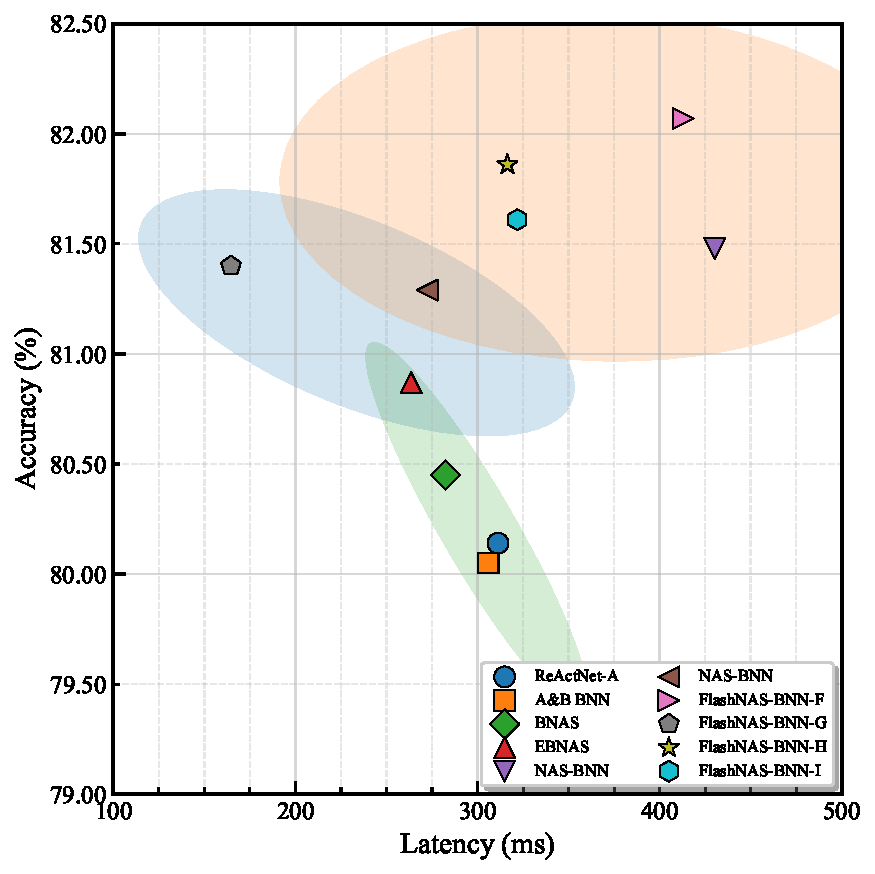
\includegraphics[height=2.3in]{./figs/Figure_7_a.pdf} & 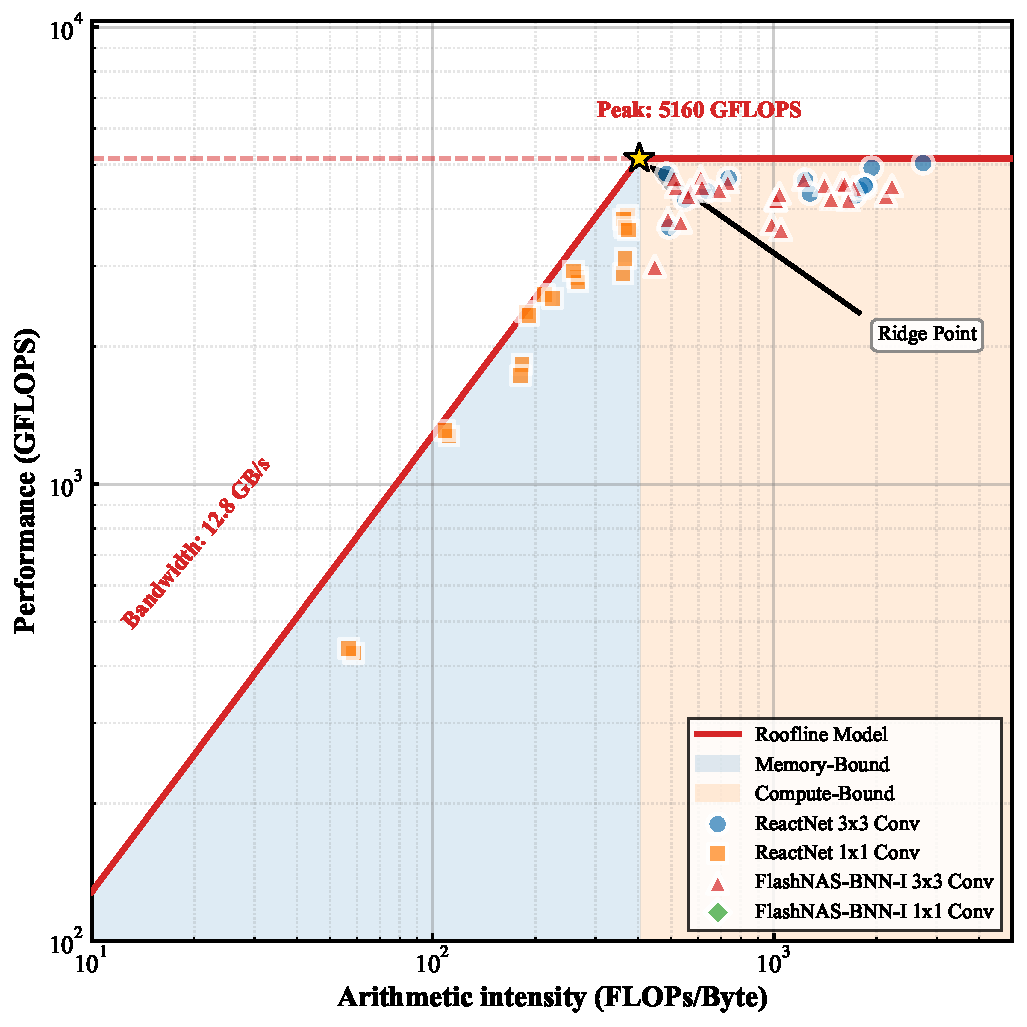
\includegraphics[height=2.3in] {./figs/Figure_7_b.pdf} \\ 
        \scriptsize (a) & \scriptsize (b)\\ 
    \end{tabular}
    \caption{Search results on ImageNet-100. (a) Accuracy-latency comparison of representative BNNs under similar computational budgets; shaded backgrounds denote cluster assignments. (b) Roofline-model comparison between the searched architecture and ReActNet.}\label{fig:7}
\end{figure}

As shown in Fig.~\ref{fig:7}(b), FlashNAS-BNN-I adopts an all-$3\times3$ convolution design with channel widths of [32, 64, 96, 192, 320, 768] and stage depths of [3, 4, 2, 4, 7, 5]. This FPGA-targeted architecture achieves 2.34\,ms/image, compared with 2.51\,ms/image for ReActNet-A (Table~\ref{tab:4}).

\subsection{\textcolor{red}{Results on search cost}}
\label{sec:search_time}
\textcolor{red}{Table~\ref{tab:search_cost} compares the search costs of FlashNAS-BNN with representative BNN NAS methods. NAS-BNN serves as the primary baseline due to its similar chain-structured search space, while cell-based methods are included for reference. For a fixed dataset and search setting, FlashNAS-BNN reuses the same CIF-Net predictor and Stage-I candidate set across target platforms, whereas NAS-BNN requires an independent search for each platform. Under this reuse setting and the accounting scheme in Table~\ref{tab:search_cost}, the cumulative costs over $M$ platforms are $T_{\text{NAS-BNN}}(M)=480M$ and $T_{\text{ours}}(M)=1363.73+0.48M$ GPU-hours. FlashNAS-BNN therefore achieves a lower cumulative search cost for three or more platforms ($M^{*}\approx2.84$). At $M=3$, the average costs are 455.06 and 480.00 GPU-hours per platform for FlashNAS-BNN and NAS-BNN, respectively, as plotted in Fig.~\ref{fig:1}(b). A separately trained predictor incurs a new offline preparation cost. For a single search, the cell-based EBNAS baseline remains less costly (Table~\ref{tab:search_cost}).}

\begin{table}[ht]
\centering
\caption{\textcolor{red}{Search cost in GPU-hours. Total includes reported offline preparation and online searches; Avg./platform is Total/$M$. FlashNAS-BNN preparation includes label generation and CIF-Net fitting. NAS-BNN supernet training and unreported baseline offline costs are excluded. Baseline searches are repeated independently per platform. A dash denotes an unreported offline cost. Detailed accounting is given in the supplementary material, ``Comparison protocols and cost accounting.}}
\label{tab:search_cost}
\small
\setlength{\tabcolsep}{4pt}
\renewcommand{\arraystretch}{1.15}

{\color{red}
\begin{tabular}{l c c c c c c c}
\toprule[1.5pt]
Method & Space & \makecell{Offline\\prep.} & \makecell{First\\online} & \makecell{Additional\\online} & \makecell{Total\\($M=1$)} & \makecell{Total\\($M=3$)} & \makecell{Avg./platform\\($M=3$)} \\
\midrule
BNAS~\cite{Kim2020} & Cell & -- & 9.60 & 9.60 & 9.60 & 28.80 & 9.60 \\
BATS~\cite{Bulat2020} & Cell & -- & 6.00 & 6.00 & 6.00 & 18.00 & 6.00 \\
EBNAS~\cite{Shi2023} & Cell & -- & 0.96 & 0.96 & 0.96 & 2.88 & 0.96 \\
UBNAS~\cite{tan2024universal} & Cell & -- & 0.96 & 0.96 & 0.96 & 2.88 & 0.96 \\
\midrule
NAS-BNN~\cite{Lin2025} & Chain & -- & 480.00 & 480.00 & 480.00 & 1440.00 & 480.00 \\
\midrule
\rowcolor{gray!20}
FlashNAS-BNN & Chain & 1363.20 & 1.01 & 0.48 & 1364.21 & 1365.17 & 455.06 \\
\bottomrule[1.5pt]
\end{tabular}
}
\end{table}

\subsection{Ablation Study}
\textcolor{red}{Table~\ref{tab:5} evaluates the contributions of CIF-Net, two-stage search, and CLE to reducing search time on ImageNet-100 relative to a direct evolutionary-search baseline.}
\begin{table}[ht]
\centering
\caption{Ablation study of different methods.}
\small
\begin{tabular}{cccccccc}
\toprule[1.5pt]
\multicolumn{1}{c}{\multirow{2}{*}{EA}} & \multicolumn{1}{c}{\multirow{2}{*}{two-stage}} & \multicolumn{1}{c}{\multirow{2}{*}{CIF-Net}} & \multicolumn{1}{c}{\multirow{2}{*}{CLE}} & \multicolumn{4}{c}{Search time (GPU-hours)} \\ 
\cmidrule{5-8} 
 & & & & StageI & StageII-10 & StageII-100 & StageII-500 \\
\midrule
\checkmark & & &       & 550.53 & - & - & -\\
\checkmark & \checkmark & &     & 528.25 & 0.02 & 0.18 & 0.96 \\
\checkmark &  & \checkmark &     & 22.81 & - & - & - \\
\checkmark &  & \checkmark &  \checkmark  & 5.64 & - & - & - \\
\checkmark & \checkmark & \checkmark &     & 0.53 & 0.02 & 0.18 & 0.96 \\
\midrule
\checkmark & \checkmark & \checkmark & \checkmark & \textbf{0.53} &  \textbf{0.02} & \textbf{0.18} & \textbf{0.48}   \\
\bottomrule[1.5pt]
\end{tabular}
\label{tab:5}
\end{table}

\subsubsection{Accuracy Predictions}
CIF-Net shows substantial search speed improvements in the first-stage of our optimization framework. As shown in Table~\ref{tab:5}, integrating CIF-Net into the EA+two-stage framework reduces the first-stage (StageI) search time from 528.25 GPU-hours to 0.53 GPU-hours, achieving a 99.90\% reduction in computational cost. Notably, the search times for subsequent stages (StageII-10, StageII-100 and StageII-500) remain consistent with those of EA+two-stage, confirming that CIF-Net specifically optimizes the initial stage without compromising downstream efficiency.
\begin{table}[ht]
\centering
\caption{Comparison of prediction accuracies for the networks.}
\small
\begin{tabular}{l l c c c c}
\toprule[1.5pt]
Dataset & Method   & MSE   & Kendall & $R^2$  & Top-1(\%) \\
\midrule
\multicolumn{1}{l}{\multirow{4}{*}{ImageNet}} & $\nu$-SVR~\cite{Baker2017}  & 0.059 & 0.747   & 0.894 & 81.87\\
~ & Peephole~\cite{Deng2017} & 0.066  & 0.763    & 0.869   & 81.64\\
~ & GCN~\cite{Qin2022} & 0.049 & 0.782   & 0.865 & 81.56\\
\cline{2-6}
~ & \textbf{Ours} & \textbf{0.022} & \textbf{0.874}   & \textbf{0.962} & \textbf{82.07}\\
\midrule
\multicolumn{1}{l}{\multirow{4}{*}{CIFAR}} & $\nu$-SVR~\cite{Baker2017}  & 0.001 & 0.3445   & -0.5420 & 93.17\\
~ & Peephole~\cite{Deng2017} & 0.0003  & 0.6545  & 0.6141 & 93.83\\
~ & GCN~\cite{Qin2022} & 0.034 & 0.1683   & -0.1749  & 93.58\\
\cline{2-6}
~ & \textbf{Ours} & \textbf{0.0003} & \textbf{0.7351}   & \textbf{0.7033} & \textbf{94.16}\\
\bottomrule[1.5pt]
\end{tabular}
\label{tab:6}
\end{table}

To further validate the effectiveness of CIF-Net in accuracy prediction, we compare it with $\nu$-SVR, Peephole, and GCN under the same OP constraint with \textcolor{red}{the accuracy-only setting $w_{\mathrm{Lat}}=1$}. The results are reported in Table~\ref{tab:6}. \textcolor{red}{The predictor metrics evaluate predictions against measured 25-epoch labels. Full-training accuracy is reported for the selected architectures. Supplementary Sections 3.1--3.2 evaluate the transfer from short-training labels to final architecture selection.}
On ImageNet, CIF-Net achieves the lowest mean squared error (MSE) of 0.022, compared with 0.059 for $\nu$-SVR, 0.066 for Peephole, and 0.049 for GCN. Relative to the best baseline (GCN), CIF-Net reduces the MSE by 0.027 (55.1\%). 
CIF-Net also yields the highest Kendall correlation (0.874), exceeding $\nu$-SVR (0.747), Peephole (0.763), and GCN (0.782). 
In terms of $R^2$, CIF-Net reaches 0.962, substantially higher than $\nu$-SVR (0.894), Peephole (0.869), and GCN (0.865), indicating a better fit between predicted and measured accuracies. Moreover, under the accuracy-only setting, the best architecture selected based on CIF-Net achieves 82.07\% Top-1 accuracy, outperforming the architectures selected by $\nu$-SVR (81.87\%), Peephole (81.64\%), and GCN (81.56\%). Qualitative visualizations of the prediction results are provided in supplementary material 4.

\begin{figure}
    \centering
    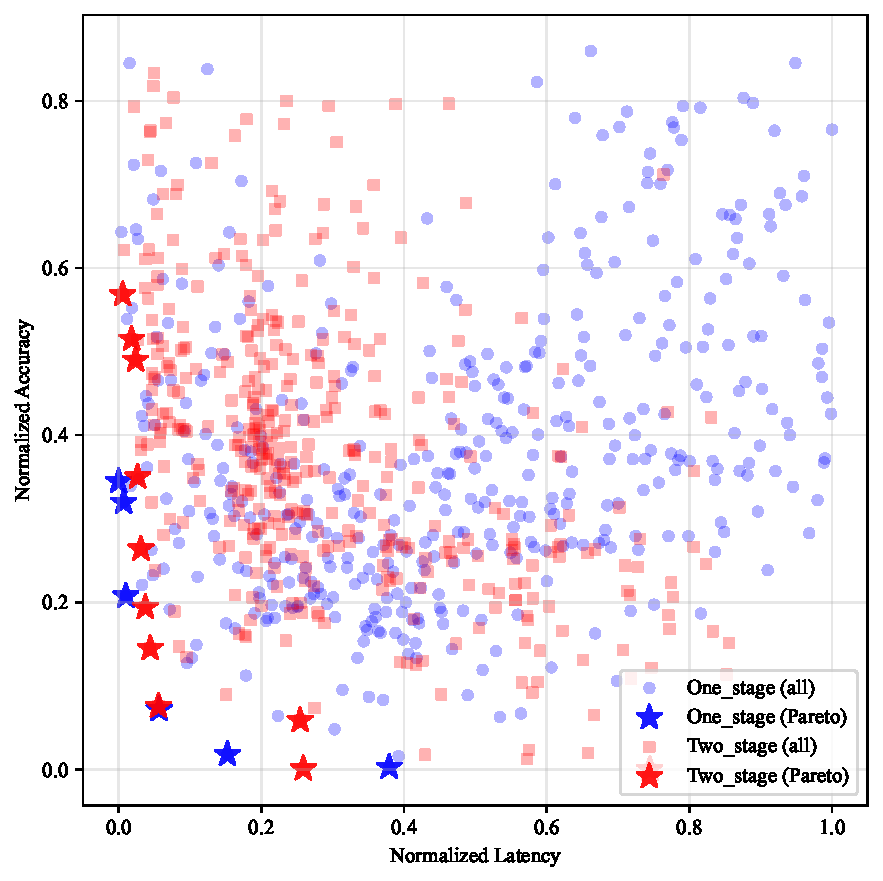
\includegraphics[height=2.5in]{./figs/Figure_8.pdf}
    \caption{Search performance results of different stage methods.}\label{fig:8}
\end{figure}

\subsubsection{Two-stage Search}
Table~\ref{tab:5} verifies that the two-stage search markedly improves search efficiency.
Compared with a one-stage evolutionary algorithm (EA) that runs Stage-I for 550.53 GPU-hours,
our two-stage design reduces the coarse Stage-I cost to 528.25 GPU-hours (4.05\%),
and adds only negligible Stage-II overhead (0.02/0.18/0.96 GPU-hours for 10/100/500 candidates).
\textcolor{red}{Reusing these Stage-I results across platforms for the same ImageNet-100 search setting saves 528.25 GPU-hours for each additional hardware target.}
Moreover, when coupled with CIF-Net, Stage-I drops to 0.53 GPU-hours\textcolor{red}{: CIF-Net alone reduces the standalone EA cost by 24$\times$ (550.53 $\rightarrow$ 22.81 GPU-hours), and the two-stage strategy reduces it by a further 43$\times$ (22.81 $\rightarrow$ 0.53 GPU-hours), giving an overall online reduction of 1038$\times$ (550.53 $\rightarrow$ 0.53 GPU-hours)}.

We further test whether two-stage search degrades the final accuracy--latency trade-off by comparing it with a one-stage baseline that directly optimizes Eq.~(\ref{eq:final_objective}) using measured CPU latency during evolution.
Both are evaluated on ImageNet-100 with a Cortex-X4 CPU (Fig.~\ref{fig:8}). Search uses each method's own candidate-set extrema; the plotted results use common post-search normalization.
The one-stage baseline explores a wider region but yields a sparse Pareto set and many solutions in the medium-to-high latency range.
By screening candidates with (accuracy, OPs) in Stage-I, our two-stage method focuses on the low-latency regime and produces a denser Pareto frontier near the left boundary, achieving a comparable accuracy--latency trade-off. Additional Pareto frontier visualizations are provided in supplementary material 5.

\begin{table}[ht]
    \centering
    \caption{\textcolor{red}{Evaluation of latency prediction and architecture selection.}}
    \small
    \begin{tabular}{llcccc}
    \toprule[1.5pt]
    \multicolumn{1}{l}{\multirow{2}{*}{Platform}} & \multicolumn{1}{l}{\multirow{2}{*}{Method}} & \multicolumn{3}{c}{Error  bound(\%)}  & \multirow{2}{*}{\makecell{\textcolor{red}{Overall chosen arch.}\\\textcolor{red}{latency (ms/image)}}}\\
    % [0.5pt] \cline{2-4} 
    \cmidrule{3-5}
    \multicolumn{1}{l}{} & \multicolumn{1}{l}{} & 1\% & 5\% & 10\% & \multicolumn{1}{c}{} \\
    \midrule
    \multicolumn{1}{l}{\multirow{7}{*}{CPU}} & Actually measured    & - & - & - & \textcolor{red}{139.97 $\pm$ 0.42} \\
    \multicolumn{1}{l}{} &\textcolor{red}{OPs Proxy} & \textcolor{red}{1.6 $\pm$ 0.8} & \textcolor{red}{9.6 $\pm$ 1.2} & \textcolor{red}{37.2 $\pm$ 1.6} & \textcolor{red}{151.78 $\pm$ 5.73} \\
    \multicolumn{1}{l}{} &$\nu$-SVR~\cite{Baker2017}      & 4.8$\pm$2.8 & 24.0$\pm$2.0 & 62.4$\pm$1.6 & \textcolor{red}{146.25 $\pm$ 2.90} \\
    \multicolumn{1}{l}{} &BRP-NAS~\cite{Dudziak2020}      & 6.8$\pm$2.0 & 21.4$\pm$2.4 & 66.0$\pm$1.2 & \textcolor{red}{145.51 $\pm$ 1.05} \\
    \multicolumn{1}{l}{} &CLCDLP~\cite{Lin2024}       & 5.2$\pm$2.4 & 18.4$\pm$2.0 & 70.8$\pm$1.2 & \textcolor{red}{143.62 $\pm$ 0.67} \\
    \multicolumn{1}{l}{} &\textcolor{red}{nn-Meter~\cite{Zhang2021nnMeter}} & \textcolor{red}{7.2 $\pm$ 2.0} & \textcolor{red}{25.2 $\pm$ 2.0} & \textcolor{red}{69.6 $\pm$ 1.6} & \textcolor{red}{142.86 $\pm$ 0.81} \\
    \cline{2-6}
    \multicolumn{1}{l}{} &\textbf{Ours}& \textbf{8.8}$\pm$2.4 & \textbf{27.4}$\pm$2.4 & \textbf{72.4}$\pm$2.0 & \textcolor{red}{\textbf{141.32} $\pm$ 0.53} \\
    \midrule
    \multicolumn{1}{l}{\multirow{7}{*}{GPU}} & Actually measured    & - & - & - & \textcolor{red}{43.78 $\pm$ 0.04} \\
    \multicolumn{1}{l}{} &\textcolor{red}{OPs Proxy} & \textcolor{red}{0.8 $\pm$ 0.4} & \textcolor{red}{8.4 $\pm$ 0.8} & \textcolor{red}{28.0 $\pm$ 1.2} & \textcolor{red}{46.07 $\pm$ 2.19} \\
    \multicolumn{1}{l}{} &$\nu$-SVR~\cite{Baker2017}      & 3.6$\pm$0.4 & 18.8$\pm$1.2 & 49.6$\pm$1.2 & \textcolor{red}{44.64 $\pm$ 0.29} \\
    \multicolumn{1}{l}{} &BRP-NAS~\cite{Dudziak2020}      & 3.8$\pm$0.4 & 22.0$\pm$1.6 & 52.4$\pm$2.0 & \textcolor{red}{44.00 $\pm$ 0.23} \\
    \multicolumn{1}{l}{} &CLCDLP~\cite{Lin2024}       & 3.2$\pm$0.8 & 23.2$\pm$1.2 & 60.8$\pm$0.8 & \textcolor{red}{44.25 $\pm$ 0.14} \\
    \multicolumn{1}{l}{} &\textcolor{red}{nn-Meter~\cite{Zhang2021nnMeter}} & \textcolor{red}{4.0 $\pm$ 0.8} & \textcolor{red}{23.6 $\pm$ 1.2} & \textcolor{red}{62.4 $\pm$ 1.6} & \textcolor{red}{44.17 $\pm$ 0.19} \\
    \cline{2-6}
    \multicolumn{1}{l}{} &\textbf{Ours}& \textbf{4.8}$\pm$1.2 & \textbf{25.2}$\pm$1.6 & \textbf{65.2}$\pm$1.6 & \textcolor{red}{\textbf{43.91} $\pm$ 0.12} \\
    \midrule
    \multicolumn{1}{l}{\multirow{7}{*}{FPGA}} & Actually measured    & - & - & - & \textcolor{red}{2.297 $\pm$ 0.004} \\
    \multicolumn{1}{l}{} &\textcolor{red}{OPs Proxy} & \textcolor{red}{1.2 $\pm$ 0.8} & \textcolor{red}{7.6 $\pm$ 1.2} & \textcolor{red}{31.2 $\pm$ 1.6} & \textcolor{red}{2.394 $\pm$ 0.075} \\
    \multicolumn{1}{l}{} &$\nu$-SVR~\cite{Baker2017}      & 12.4$\pm$3.6 & 36.0$\pm$2.4 & 79.2$\pm$1.2 & \textcolor{red}{2.310 $\pm$ 0.008} \\
    \multicolumn{1}{l}{} &BRP-NAS~\cite{Dudziak2020}      & 13.2$\pm$2.4 & 39.2$\pm$2.0 & 81.6$\pm$0.8 & \textcolor{red}{2.310 $\pm$ 0.009} \\
    \multicolumn{1}{l}{} &CLCDLP~\cite{Lin2024}       & 14.4$\pm$3.2 & 38.8$\pm$2.8 & 83.6$\pm$1.2 & \textcolor{red}{2.320 $\pm$ 0.007} \\
    \multicolumn{1}{l}{} &\textcolor{red}{nn-Meter~\cite{Zhang2021nnMeter}} & \textcolor{red}{14.0 $\pm$ 2.8} & \textcolor{red}{39.6 $\pm$ 2.0} & \textcolor{red}{82.4 $\pm$ 1.6} & \textcolor{red}{2.309 $\pm$ 0.007} \\
    \cline{2-6}
    \multicolumn{1}{l}{} &\textbf{Ours}& \textbf{20.8}$\pm$4.0 & \textbf{46.0}$\pm$2.4 & \textbf{92.4}$\pm$1.2  & \textcolor{red}{\textbf{2.300} $\pm$ 0.005} \\
    \bottomrule[1.5pt]
    \end{tabular}
    \label{tab:7}
\end{table}

\subsubsection{CLE}
The results in Table~\ref{tab:5} demonstrate that CLE is crucial for reducing search cost.
Under the EA + two-stage + CIF-Net framework, CLE halves the StageII-500 time from 0.96 to 0.48 GPU-hours.
Consequently, the full pipeline (StageI + StageII-500) takes 1.01 GPU-hours, a 32.2\% reduction from 1.49 GPU-hours without CLE, validating its effectiveness in accelerating NAS. \textcolor{red}{The threshold selection for Stage-II latency evaluation is provided in Section 7.1 of the supplementary material.}

We further validate CLE with \emph{measured} latencies on CPU/GPU/FPGA, with the same OP constraint and \textcolor{red}{the latency-only setting $w_{\mathrm{Lat}}=0$} (Table~\ref{tab:7}).
\textcolor{red}{Error-bound percentages count predictions within 1\%, 5\%, or 10\% relative error. Actually measured denotes hardware-guided search. Selected architectures are timed on hardware; error-bound percentages and Overall selected-architecture latency report mean $\pm$ sample SD across three searches. Per-search measurements and seeds are given in Supplementary Section 7.2.}
\textcolor{red}{On CPU, CLE achieves a selected-architecture latency of $141.32\pm0.53$\,ms, compared with $146.25\pm2.90$\,ms for $\nu$-SVR, $145.51\pm1.05$\,ms for BRP-NAS, and $143.62\pm0.67$\,ms for CLCDLP; the Actually measured baseline yields $139.97\pm0.42$\,ms. On GPU, CLE yields $43.91\pm0.12$\,ms, compared with $43.78\pm0.04$\,ms for Actually measured. On FPGA, CLE yields $2.300\pm0.005$\,ms, compared with $2.297\pm0.004$\,ms for Actually measured; their mean latency gap is 0.003\,ms. CLE also achieves the highest within-bound latency prediction accuracy on CPU (8.8\%/27.4\%/72.4\% for 1\%/5\%/10\%). On GPU, the corresponding proportions are 4.8\%/25.2\%/65.2\%, and on FPGA they are 20.8\%/46.0\%/92.4\%.}


\section{Conclusion}
In this paper, we presented FlashNAS-BNN, an efficient chain-structured binary neural architecture search framework for visual recognition across heterogeneous platforms. Building on the chain-structured NAS paradigm, FlashNAS-BNN improves efficiency in two complementary aspects: search efficiency and deployment efficiency. Specifically, it integrates an accuracy predictor, a decoupled two-stage search strategy, and a cross-platform latency estimation mechanism to accelerate architecture search while identifying latency-optimized BNNs for diverse hardware platforms. Extensive experiments on edge devices demonstrate that FlashNAS-BNN supports efficient platform-specific online search and \textcolor{red}{reduces inference latency by 6.8\%--47.1\% relative to ReActNet-A and by 8.6\%--39.6\% relative to the corresponding platform-optimized NAS-BNN architectures on the evaluated CPU, GPU, and FPGA platforms, at comparable accuracy}. \textcolor{red}{Including offline preparation, cumulative search cost becomes lower than independent NAS-BNN searches for three or more platforms under the reuse setting in Sec.~\ref{sec:search_time}.} These results highlight the practical value of FlashNAS-BNN for rapidly generating device-specific BNN models in latency-sensitive and resource-constrained visual applications. In future work, we will extend the framework to broader visual recognition tasks, larger search spaces, and a wider range of heterogeneous edge platforms, with the goal of enabling more efficient deployment of vision models in real-world scenarios.

\appendix
\section{Supplementary material}
This supplementary material provides the experimental setup and latency measurement protocol, followed by additional results and discussions on the search algorithm, cross-platform latency estimation, accuracy prediction, Pareto frontier comparison, weight coefficients, and Stage-II latency evaluation.

\printcredits

\section*{Declaration of generative AI and AI-assisted technologies in the 
writing process}
During the preparation of this work the authors used ChatGPT in order to improve readability and language. After using this tool, the authors reviewed and edited the content as needed and take full responsibility for the content of the publication.

\section*{Declaration of competing interest}
The authors declare that they have no known competing financialinterests or personal relationships that could have appeared to influencethe work reported in this paper.

\section*{Acknowledgments}
This research was sponsored by Beijing Natural Science Foundation grant number L244050 and L252018.

\section*{Data availability}
All datasets used in this study are publicly available benchmark datasets.

%% Loading bibliography style file
%\bibliographystyle{model1-num-names}
\bibliographystyle{cas-model2-names}

% Loading bibliography database
\bibliography{cas-refs}


%\vskip3pt


\end{document}

